\chapter{Model błędu wyniku pomiaru}

Aby określić w jakim stopniu analizowany tor pomiarowy spełnia powierzone mu zadanie pomiarowe należy ilościowo przedstawić przedział, w którym z określonym prawdopodobieństwem będą znajdowały się wartości wielkości wyjściowych tego toru pomiarowego~\cite{jcgm_guide}. Należy zatem zdefiniować w jaki sposób rozumiana jest idealna wartość wielkości wyjściowej, a następnie zdefiniować różnicę pomiędzy rzeczywistą i idealną wartością wielkości wyjściowej nazywaną w dalszej części pracy błędem wielkości wyjściowej. Zakładając, że proces uzyskiwania wartości wielkości wyjściowej będzie powtarzany wielokrotnie, opisaną różnicę można analizować probabilistycznie, przedstawiając jej parametry za pomocą funkcji gęstości prawdopodobieństwa. W przypadku, gdy analizowany tor pomiarowy dostarcza na wyjściu wiele wielkości wyjściowych, każdą z nich należy analizować osobno. Istnieją jednak przypadki, w których analiza może odbywać się zbiorczo dla pewnej grupy wielkości wyjściowych, wykazującej identyczne właściwości metrologiczne.

Analizując tor pomiarowy przedstawiony na rysunku~\ref{fig:chain_demo} zauważyć można, że w pierwszej fazie przetwarzania wielkości wejściowej $s(t)$ wielkość ta jest ciągła w dziedzinie czasu. Wielkość wyjściowa $y(t)$ części analogowej jest efektem przetwarzania wielkości wyjściowej $s(t)$ zgodnie z charakterystyką tej części, przy czym jej właściwości mogą zależeć od widma przetwarzanego sygnału. Aby ujednolicić analizę cześć analogowej, jej właściwości należy zatem rozpatrywać nie w dziedzinie czasu, a w dziedzinie częstotliwości. Właściwości analogowej część toru pomiarowego, zależne od częstotliwości przetwarzanego przez nią sygnału, mogą być zatem opisane za pomocą transmitancji $G(j\omega)$. Analogicznie postąpić można w przypadku cyfrowej cześć toru pomiarowego. Właściwości części cyfrowej, uzależnione od widma przetwarzanego przez nią sygnału, opisać można za pomocą transmitancji $H(z)$. Każda z omawianych części, poza odpowiednio wyrażona transmitancją, charakteryzuje się związaną z nią funkcją przetwarzania oznaczoną symbolem $f(x)$. Funkcja ta opisuje w jaki sposób element wyznacza wartość wielkości wyjściowej na podstawie wartości wielkości wejściowej. Pomiędzy częściami analogową i cyfrową znajduje się przetwornik analogowo-cyfrowy. Schemat ideowy dla omawianego przypadku z punktu widzenia pojedynczej wielkości wyjściowej toru pomiarowego przedstawiono na rysunku~\ref{fig:chain_trans}.

\begin{figure}[htb!]
\begin{center}
\includegraphics{obrazki/schemat_trans}
\makecaption{fig:chain_trans}{Schemat blokowy toru pomiarowego z punktu widzenia pojedynczej wielkości wyjściowej}
\end{center}
\end{figure}

Przedstawiony na rysunku~\ref{fig:chain_trans} przypadek zakłada, że przetwarzanie analogowo-cyfrowe przebiega w sposób idealny, tj. wprowadza do przetwarzanego sygnału jedynie błąd związany z procesem kwantowania wartości wielkości wejściowych. Założenie to będzie oczywiście nieprawidłowe w rzeczywistym torze pomiarowym, dlatego sam przetwornik analogowo-cyfrowy również należy opisać za pomocą przedstawionego na rysunku~\ref{fig:chain_trans} modelu o parametrach odpowiednich dla analizowanego przetwornika. Naturalnie, tor pomiarowy składać się może z wielu elementów połączonych ze sobą szeregowo, które odpowiednio przetwarzać będą sygnał ciągły w czasie lub przetwarzać będą jego dyskretną reprezentacje. Należy zatem przedstawiać rzeczywisty tor pomiarowy jako połączenie kolejnych elementów o odpowiednich dla nich parametrach lub za pomocą modelu opisującego wypadkowe parametry wszystkich analizowanych części tego toru. W przypadku, gdy dla analizowanego fragmentu toru pomiarowego jego właściwości nie są istotne z punktu analizy metrologicznej, właściwości te można pominąć.

Analizując właściwości metrologiczne elementów toru pomiarowego należy dokonać podziału ich cech ze względu na rolę w przetwarzaniu przez nie sygnału wejściowego. Część cech będzie bowiem użyteczna z punktu widzenia roli toru pomiarowego (np. wzmocnienie sygnału, filtracja sygnału), przy czym te same cechy mogą okazać się problematyczne i wprowadzać będą one do wielkości wyjściowej niepożądane z punktu widzenia realizowanego zadania błędy (np. filtracja sygnału, gdy nie jest pożądana, będzie ten sygnał tłumić i przesuwać w fazie). Każdy z fragmentów toru pomiarowego, zgodnie ze swoimi właściwościami, wprowadzać będzie do sygnału wyjściowego błędy własne oraz przenosić będzie na wyjście obecne w sygnale wejściowym błędy. Jak wcześniej wspomniano, nie wszystkie właściwości analizowanego elementu toru pomiarowego będą odpowiedzialne za wprowadzanie do wielkości wyjściowych błędów -- jeśli ich działanie jest pożądane, to przyjmuje się że realizują powierzone im zadanie przetwarzania sygnału. Dla przykładu, jeśli elementem toru pomiarowego jest wzmacniacz, to jego zadaniem jest wprowadzenie stałego wzmocnienia wielkości wejściowych niezależnie od widma sygnału wejściowego. Jeśli zatem element ten wprowadzi inne wzmocnienie, niż oczekiwane, lub też wpłynie on na widmo przetwarzanego sygnału, działanie to zostanie rozpatrzone jako niepożądane, a jego skutki zostaną opisane jako wprowadzenie błędu własnego do wielkości wyjściowej. Z drugiej strony, jeśli analizowanym elementem byłby filtr, to wprowadzenie tłumienia byłoby działaniem pożądanym i nie zostałoby opisane jako wprowadzenie błędu własnego do przetwarzanego sygnału -- chyba, że wprowadzone tłumienie posiadałoby parametry inne, niż oczekiwane. Należy zatem analizować właściwości kolejnych fragmentów toru pomiarowego w taki sposób, aby ocenić ich działanie pod kątem powierzonego im zadania przetworzenia wielkości wejściowych, a następnie określić, które ich cechy są pożądane, a które nie.

Ze względu na charakter, właściwości każdego z fragmentów toru pomiarowego podzielić można na dwie najważniejsze grupy:
\begin{description}
\item [Właściwości statyczne] w przypadku, gdy właściwości te nie są związane z widmem przetwarzanego sygnału wejściowego.
\item [Właściwości dynamiczne] w przypadku gdy właściwości te są bezpośrednio związane z widmem przetwarzanego sygnału.
\end{description}

Jako, że wybrane właściwości kolejnych fragmentów toru pomiarowego będą zależały od widma przetwarzanego sygnału, w dalszej cześć rozdziału przyjmuje się założenie, że niezakłócony błędami przetwarzany sygnał wejściowy $s(t)$ opisać można w postaci sumy kolejnych harmonicznych tego sygnału równaniem:
\begin{equation}
\dot{s} \emb{t} = \sum _{i = 0} ^{\infty} \dot{s} \left( t, \omega_{s,i} \right) \label{eq:in_cont_sum},
\end{equation}
przy czym $\omega_{s,i}$ jest pulsacją $i$-tej harmonicznej opisywanego sygnału oraz:
\begin{gather}
\dot{s} \left( t, \omega \right) = E_{s,o} \emb{\omega} \sin \left( \omega t + \varphi_{s,o} \emb{\omega} \right) \label{eq:in_cont_omega_ideal}, \\
\tilde{s} \left( t, \omega \right) = \dot{s} \left( t, \omega \right) + E_{s,e} \emb{\omega} \sin \left( \omega t + \varphi_{s,e} \emb{\omega} \right) \label{eq:in_cont_omega_real}, \\
\tilde{s} \emb{t} = e_{s,r} \emb{t} + \sum _{i = 0} ^{\infty} \tilde{s} \left( t, \omega_{s,i} \right) \label{eq:in_cont_sum_real},
\end{gather}
gdzie $E_{s,o}(\omega)$ jest amplitudą oraz $\varphi_{s,o}(\omega)$ przesunięciem w fazie wybranej harmonicznej sygnału, $E_{s,e}$ amplitudą oraz $ \varphi_{s,e}$ przesunięciem w fazie analizowanej harmonicznej przebiegu błędu zawartego w sygnale, natomiast $e_{s,r}$ jest błędem losowym. W opisie sygnału pominięto jawny opis składowej stałej sygnału, jako że zastąpić go można harmoniczną o indeksie $i = 0$, gdzie $\omega_{0} = 0$ oraz $\varphi_{0} = \pi$.

Na podstawie równania~\eqref{eq:in_cont_omega_real} wyróżnić można trzy grupy błędów, przy czym zaproponowany podział wynika z charakteru ich realizacji i obejmuje:
\begin{description}
\item [Błędy statyczne] dla których kolejne realizacje w obrębie pojedynczego okna pomiarowego nie zmieniają się lub zmieniają się nieznacznie.
\item [Błędy dynamiczne] dla których kolejne realizacje można opisać w sposób deterministyczny, jako sumę kolejnych harmonicznych tego błędu.
\item [Błędy losowe] dla których kolejne realizacje będą wynikały z reguł probabilistycznych, a zatem ich opis deterministyczny nie będzie możliwy.
\end{description}

Analizując przedstawione powyżej założenia oraz biorąc pod uwagę równania od~\eqref{eq:in_cont_sum} do~\eqref{eq:in_cont_sum_real}, wyróżnione błędy deterministyczne opisać można za pomocą równań:
\begin{gather}
e_{s,s} \emb{t} = E_{s,e} \emb{\omega_{s,0}} \sin \left( \omega_{s,0} t + \varphi_{s,e} \emb{\omega_{s,0}} \right) = E_{s,e} \emb{0} \label{eq:in_cont_err_stat}, \\
e_{s,d} \emb{t} = \sum _{i = 1} ^{\infty} E_{s,e} \emb{\omega_{s,i}} \sin \left( \omega_{s,i} t + \varphi_{s,e} \emb{\omega_{s,i}} \right) \label{eq:in_cont_err_dyn},
\end{gather}
gdzie symbolem $e_{s,s}$ oznaczono błąd statyczny, natomiast symbolem $e_{s,d}$ błąd dynamiczny zawarty w sygnale $s(t)$. Błąd wypadkowy $e_{s,\Sigma}$ zawarty w sygnale $s(t)$ można zatem wyrazić w postaci sumy wszystkich wymienionych błędów:
\begin{equation}
e_{s,\Sigma} \emb{t} = e_{s,s} \emb{t} + e_{s,d} \emb{t} + e_{s,r} \emb{t} \label{eq:in_cont_err_sum}.
\end{equation}

\section{Błędy w części analogowej toru pomiarowego}

Aby ujednolicić analizę pojedynczego fragmentu części analogowej toru pomiarowego, element ten można przedstawić za pomocą transmitancji operatorowej odpowiadającej właściwościom dynamicznym, przy czym wzmocnienie tej części będzie równe jedności, oraz opisać właściwości statyczne w postaci odpowiedniej dla analizowanego obiektu funkcji przetwarzania. Na rysunku~\ref{fig:chain_cont} przedstawiono schemat fragmentu toru pomiarowego zbudowany w opisywany sposób. W dalszej części podrozdziału zakłada się, że analizowany fragment toru pomiarowego przetwarza ciągły w czasie sygnał $s(t)$, opisany we wstępie rozdziału równaniami od~\eqref{eq:in_cont_sum} do~\eqref{eq:in_cont_sum_real}, na sygnał $y(t)$. Dodatkowo przyjmuje się, że funkcja $f_{y}(x)$ stanowi równanie przetwarzania opisywanego obiektu, natomiast transmitancja obiektu jest wyrażona jako $G_{u}(j\omega)$, przy czym jej wzmocnienie jest równe jedności, a jej charakter jest liniowy i nie zależny w żaden sposób od czasu.

\begin{figure}[htb!]
\begin{center}
\includegraphics{obrazki/schemat_ciagly}
\makecaption{fig:chain_cont}{Schemat blokowy pojedynczego fragmentu części analogowej toru pomiarowego}
\end{center}
\end{figure}

Błędy obecne w sygnale wyjściowym $y(t)$ podzielić można, podobnie jak we wprowadzeniu do rozdziału, na statyczne, dynamiczne i losowe. Podział ten natomiast należy rozszerzyć pod kątem genezy błędu, przy czym wyróżnione zostaną w tym przypadku błędy własne oraz propagowane. Błędy własne to takie, które analizowany obiekt wprowadza do sygnału wyjściowego. Błędy propagowane są natomiast błędami zawartymi w sygnale wejściowym, przetworzonymi przez obiekt zgodnie z jego charakterystyką, a następnie przeniesionymi na wyjście tego obiektu. Suma błędów własnych i propagowanych dla danej grupy błędów stanowi błąd wypadkowy.

W pierwszej kolejności omówiony zostanie wpływ transmitancji $G_{u}(j\omega)$ analizowanego obiektu na błędy zawarte w wielkości wejściowej oraz jej rola we wprowadzaniu błędów własnych. W przypadku błędów statycznych, zgodnie z wprowadzonymi założeniami, transmitancja ta nie ma żadnego wpływu na obecne w sygnale wejściowym błędy statyczne oraz nie wprowadza własnego błędu statycznego. Można zatem zapisać, że:
\begin{gather}
e_{u,sw} \emb{t} = 0 \label{eq:mid_cont_err_stat_self}, \\
e_{u,sp} \emb{t} = E_{s,s} \emb{0} \label{eq:mid_cont_err_stat_prop},
\end{gather}
gdzie $e_{u,sw}$ jest błędem własnym, a $e_{u,sp}$ błędem przenoszonym przez fragment obiektu związany z jego właściwościami dynamicznymi.

Na podstawie transmitancji widmowej $G_{u}(j\omega)$ obiektu wyznaczyć można wzmocnienie $K_{u}(\omega)$ tego obiektu w funkcji pulsacji równe:
\begin{equation}
K_{u} \emb{\omega} = \left| G_{u} \emb{j\omega} \right| =
	\sqrt{\left( \Re \left( G_{u} \emb{j\omega} \right) \right)^{2} +
	\left( \Im \left( G_{u} \emb{j\omega} \right) \right)^{2}}
\label{eq:mid_cont_amp},
\end{equation}
oraz przesunięcie w fazie $\varphi_{u}(\omega)$ dla wybranej harmonicznej sygnału wejściowego dane zależnością:
\begin{equation}
\varphi_{u} \emb{\omega} = \arctan \left( \frac{\Im \left( G_{u} \emb{j\omega} \right)}{\Re \left( G_{u} \emb{j\omega} \right)} \right) \label{eq:mid_cont_phi}.
\end{equation}
Znajomość tych parametrów będzie niezbędna do opisu błędów dynamicznych własnych oraz propagowanych dla części związanej z transmitancją obiektu. Można zauważyć, że bezpośrednia znajomość transmitancji widmowej obiektu nie jest konieczna, jeśli znane są przebiegi przedstawionych parametrów w funkcji częstotliwości.

Wprowadzanie przez analizowany obiekt błędów dynamicznych wynika z faktu, że rzeczywista transmitancja $\tilde{G}_{u}(j\omega)$ odbiega od transmitancji idealnej $\dot{G}_{u}(j\omega)$. Powoduje to, że obiekt ten wprowadza inne tłumienie i przesunięcie w fazie do kolejnych harmonicznych sygnału, niż wymagane dla realizowanego przez niego zadania pomiarowego. Rozpatrując pojedynczą harmoniczną sygnału $u(t)$, można opisać idealny przebieg tej harmonicznej w postaci równania:
\begin{equation}
\dot{u} \emb{t,\omega} = \dot{K}_{u} \emb{\omega} E_{s,o} \emb{\omega} \sin \left( \omega t + \varphi_{s,o} \emb{\omega} + \dot{\varphi}_{u} \emb{\omega} \right) \label{eq:mid_cont_omega_ideal},
\end{equation}
natomiast ten sam przebieg zakłócony błędami własnym i propagowanymi, wynikającymi z transmitancji obiektu, wyrazić można w postaci równania:
\begin{equation}
\begin{split}
\tilde{u} \emb{t,\omega} =~
& \tilde{K}_{u} \emb{\omega} E_{s,o} \emb{\omega} \sin \left( \omega t + \varphi_{s,o} \emb{\omega} + \tilde{\varphi}_{u} \emb{\omega} \right) + \\
& \tilde{K}_{u} \emb{\omega} E_{s,e} \emb{\omega} \sin \left( \omega t + \varphi_{s,e} \emb{\omega} + \tilde{\varphi}_{u} \emb{\omega} \right)
\end{split}
\label{eq:mid_cont_omega_real},
\end{equation}
Wobec powyższych zależności, wprowadzany do sygnału $u(t)$ błąd dynamiczny własny $e_{u,dw}$ opisać można równaniem:
\begin{equation}
\begin{split}
e_{u,dw} \emb{t} =~
& \sum _{i = 1} ^{\infty} \tilde{K}_{u} \emb{\omega_{s,i}} E_{s,o} \emb{\omega_{s,i}} \sin \left( \omega_{s,i} t + \varphi_{s,o} \emb{\omega_{s,i}} + \tilde{\varphi}_{u} \emb{\omega_{s,i}} \right) - \\
& \sum _{i = 1} ^{\infty} \dot{K}_{u} \emb{\omega_{s,i}} E_{s,o} \emb{\omega_{s,i}} \sin \left( \omega_{s,i} t + \varphi_{s,o} \emb{\omega_{s,i}} + \dot{\varphi}_{u} \emb{\omega_{s,i}} \right)
\end{split}
\label{eq:mid_cont_err_dyn_self}.
\end{equation}
Poza wprowadzaniem do sygnału $u(t)$ błędu dynamicznego własnego, analizowany fragment obiektu przenosi z wejścia na wyjście błędy zawarte w sygnale wejściowym odpowiednio tłumiąc je i przesuwając w fazie:
\begin{equation}
e_{u,dp} \emb{t} = \sum _{i = 1} ^{\infty} \tilde{K}_{u} \emb{\omega_{s,i}} E_{s,e} \emb{\omega_{s,i}} \sin \left( \omega_{s,i} t + \varphi_{s,e} \emb{\omega_{s,i}} + \tilde{\varphi}_{u} \emb{\omega_{s,i}} \right) \label{eq:mid_cont_err_dyn_prop},
\end{equation}
przy czym $e_{u,dp}$ jest błędem dynamicznym analizowanego obiektu, propagowanym z wejścia na wyjście fragmentu reprezentującego właściwości dynamiczne tego obiektu.

Ostatnią grupą błędów dla analizowanego fragmentu obiektu stanowią błędy losowe. Błędów tych nie sposób opisać równaniem deterministycznym, a zatem opis ich właściwości sprowadzać się będzie do wskazania prawdopodobieństwa uzyskania wybranych wartości kolejnych realizacji tych błędów. W dalszej cześć podrozdziału przyjęte zostanie założenie, że $\sigma_{s,r}^{2}$ jest wariancją, a $\sigma_{s,r}$ odchyleniem standardowym błędu losowego zawartego w przetwarzanym sygnale wejściowym, oraz że kolejne wartości realizacji tego błędu nie są ze sobą skorelowane. Dodatkowo przyjmuje się, że widmowa gęstość mocy analizowanego błędu jest stała i wynosi $\sigma_{s,r}^{2}$. Wobec powyższych założeń zauważyć można, że wpływ transmitancji $G_{u}(j\omega)$ na sygnał błędu losowego zaowocuje pojawieniem się korelacji pomiędzy kolejnymi realizacjami błędu wyjściowego, co w efekcie spowoduje, że wyjściowy sygnał błędu będzie mógł być zyskać opis deterministyczny~\cite{bibbona_filter, benassi_filter}.

Przedstawione zjawisko znacznie utrudnia analizę błędów losowych. Zważywszy, że w praktyce każdy element toru pomiarowego posiada transmitancję różną od $G(j\omega) = \text{const}$, w zasadzie na jego wyjściu nigdy nie otrzymuje się sygnału błędu o przedstawionych w poprzednim akapicie założeniach. Aby umożliwić analizę dla błędów losowych, w przypadku gdy są one przetwarzane przez rzeczywisty obiekt, zaproponowana zostanie metoda pozwalająca na oszacowanie wariancji tych błędów uwzględniająca transmitancje obiektu oraz wariancję błędu na wejściu obiektu. Szacowaną wartość wariancji $\sigma_{u,rp}^{2}$ błędu losowego na wyjściu obiektu opisać można równaniem~\cite{jadziak_dsp, proakis_dsp}:
\begin{equation}
\sigma_{u,rp}^{2} = \frac{1}{a - b} \int _{b} ^{a} \tilde{K}_{u}^{2} \emb{\omega} \sigma_{s,r}^{2} d\omega \label{eq:mid_cont_var_rand},
\end{equation}
przy czym $<a;b>$ jest zakresem częstotliwości, dla którego szacowana jest wariancja przenoszonego błędu losowego. W przypadku wystąpienia błędów losowych własnych również należy wskazać ich wariancję, opisaną jako $\sigma_{u,rw}^{2}$.

Ostatecznie, sumując wszystkie błędy wielkości wyjściowej analizowanej części właściwości dynamicznych obiektu, otrzymuje się zależność określającą błąd wypadkowy $e_{u,\Sigma}$ opisaną równaniem:
\begin{equation}
e_{u,\Sigma} \emb{t} = e_{u,sp} \emb{t} + e_{u,dw} \emb{t} + e_{u,rw} \emb{t} + e_{u,dp} \emb{t} + e_{u,rp} \emb{t} \label{eq:mid_cont_err_sum_all}.
\end{equation}
Uwzględniając równanie przetwarzania $f_{y}$ analizowanego obiektu zapisać można równanie przedstawiające idealną wielkość wyjściową obiektu jako:
\begin{equation}
\dot{y} \emb{t} = \dot{f}_{y} \left( \dot{s} \emb{t} \right) \label{eq:out_cont_ideal_all},
\end{equation}
natomiast, przy uwzględnieniu równania~\eqref{eq:mid_cont_err_sum_all}, wielkość obarczoną omówionymi błędami zapisać można w postaci:
\begin{equation}
\tilde{y} \emb{t} = \tilde{f}_{y} \left( \dot{s} \emb{t} + e_{u,\Sigma} \emb{t} \right) = \dot{y} \emb{t} + e_{y,\Sigma} \emb{t} \label{eq:out_cont_real_all}.
\end{equation}
Wypadkowy błąd wielkości wyjściowej analizowanego obiektu jest zatem dany równaniem:
\begin{equation}
e_{y,\Sigma} \emb{t} = \tilde{f}_{y} \left( \dot{s} \emb{t} + e_{u,\Sigma} \emb{t} \right) - \dot{f}_{y} \left( \dot{s} \emb{t} \right) + f_{z} \left( z_{1}, \hdots, z_{N} \right) \label{eq:out_cont_err_sum_all},
\end{equation}
przy czym $\tilde{f}_{y}$ jest rzeczywistym, $\dot{f}_{y}$ idealnym równaniem przetwarzania analizowanego obiektu, natomiast $f_{z}(\mathbf{z})$ funkcją uwzględniającą wybrane wielkości zakłócające.

Przypadek ogólny, przedstawiony w równaniach od~\eqref{eq:out_cont_ideal_all} do~\eqref{eq:out_cont_err_sum_all}, jest w praktyce trudny do analizowania. Nie gwarantuje on bowiem możliwości analizy każdego błędu cząstkowego z osobna i nie będzie szczegółowo analizowany w niniejszej pracy. Dla przypadków, w których funkcja przetwarzania $f_{y}$ jest addytywna, tj. spełnia założenie $f_{y}(a + b) = f_{y}(a) + f_{y}(b)$, gdzie $a$ oraz $b$ należą do dziedziny tej funkcji, opisywaną analizę można przeprowadzić z osobna dla każdego rodzaju błędów. Przedstawione założenie jest w praktyce często spełniane, ponieważ funkcja przetwarzania reprezentuje zwykle czułość obiektu w przypadku obiektów o charakterze liniowym, a zatem jest ona funkcją liniową wyrażoną w postaci równania $f(x) = ax$, gdzie współczynnik $a$ jest czułością obiektu. W dalszej części podrozdziału zostanie przyjęte powyższe założenie dotyczące addytywności funkcji $f_{y}$, a następnie przedstawione zostaną zależności wynikające z tego założenia.

W przypadku, gdy funkcja przetwarzania nie jest idealna lub gdy istnieją pewne wielkości zakłócające niebrane pod uwagę podczas pomiaru (np. wpływ ciśnienia, temperatury itp.), natomiast nie zmieniają się one w trakcie wykonywania pomiarów, wyróżnić można dodatkowy wprowadzany błąd własny. Jeśli błąd ten nie będzie zależny od widma sygnału wejściowego, to sklasyfikować go można jako błąd statyczny i opisać symbolem $e_{y,sw}$. Przebieg tego błędu określa równanie:
\begin{equation}
e_{y,sw} \emb{t} = \tilde{f}_{y} \left( E_{s,o} \emb{0} \right) - \dot{f}_{y} \left( E_{s,o} \emb{0} \right) + f_{z} \left( z_{1}, \hdots, z_{N} \right) \label{eq:out_cont_err_stat_self},
\end{equation}
gdzie $\tilde{f}_{y}(x)$ jest rzeczywistą, a $\dot{f}_{y}(x)$ idealną funkcją przetwarzania analizowanego obiektu. Pozostałe błędy, przy założeniu addytywności funkcji przetwarzania, opisać można za pomocą równań:
\begin{gather}
e_{y,sp} \emb{t} = \tilde{f}_{y} \left( e_{u,sp} \emb{t} \right) \label{eq:out_cont_err_stat_prop}, \\
e_{y,dw} \emb{t} = \tilde{f}_{y} \left( e_{u,dw} \emb{t} \right) \label{eq:out_cont_err_dyn_prop}, \\
e_{y,dp} \emb{t} = \tilde{f}_{y} \left( e_{u,dp} \emb{t} \right) \label{eq:out_cont_err_dyn_self}, \\
e_{y,rw} \emb{t} = \tilde{f}_{y} \left( e_{u,rw} \emb{t} \right) \label{eq:out_cont_err_rand_self}, \\
e_{y,rp} \emb{t} = \tilde{f}_{y} \left( e_{u,rp} \emb{t} \right) \label{eq:out_cont_err_rand_prop},
\end{gather}
przy czym kolejno $e_{y,sp}$ jest błędem statycznym propagowanym, $e_{y,dw}$ błędem dynamicznym własnym, $e_{y,dp}$ błędem dynamicznym propagowanym oraz $e_{y,rp}$ błędem losowym propagowanym wielkości wyjściowej obiektu. Wobec powyższych równań i przyjętych założeń, równanie~\eqref{eq:out_cont_err_sum_all} przyjmuje postać:
\begin{equation}
e_{y,\Sigma} \emb{t} = e_{y,sw} \emb{t} + e_{y,sp} \emb{t} + e_{y,dw} \emb{t} + e_{y,dp} \emb{t} + e_{y,rw} \emb{t} + e_{y,rp} \emb{t} \label{eq:out_cont_err_sum_add}.
\end{equation}

Analizując przedstawione powyżej równania zauważyć można kluczowy wpływ funkcji przetwarzania $f_{y}$ obiektu na wprowadzane i przenoszone błędy. W przypadku nieliniowej charakterystyki przetwarzania obiektu, dla kolejnych harmonicznych przetwarzanego sygnału oraz harmonicznych błędu mogą pojawić się dodatkowe, wprowadzane przez funkcję przetwarzania harmoniczne. Dla liniowej funkcji przetwarzania rolę tej funkcji zastąpić można wzmocnieniem zawartym w transmitancji analizowanego obiektu i pominąć jej udział w dalszych rozważaniach.

Podsumowując przedstawione zależności zauważyć można, że przedstawiona dla błędów statycznych analiza jest szczególnym przypadkiem analizy dla błędów dynamicznych, w którym analizowany fragment toru pomiarowego przetwarza sygnał stały lub na tyle wolno-zmienny, że jego właściwości dynamiczne nie mają żadnego wpływu na przetwarzany sygnał. W przypadku propagowanych przez obiekt błędów dynamicznych, jeśli transmitancja analizowanego obiektu nie wpływa znacząco na ich widmo, to są one przenoszone zgodnie z charakterystyką statyczną obiektu. Dodatkowo, w przypadku gdy transmitancja obiektu nie wpływa w żaden sposób na widmo przetwarzanego sygnału, obiekt nie będzie wprowadzał do sygnału wyjściowego błędów dynamicznych własnych.

\section{Błędy przetwornika analogowo-cyfrowego}

Pomiędzy częściami analogową i cyfrową w torze pomiarowym znajduje się przetwornik, który przekształca ciągły sygnał wejściowy na jego dyskretną reprezentację. Można zatem stwierdzić, że element ten zaokrągla przetwarzaną wartość sygnału wejściowego do najbliższej wartości będącej wielokrotnością liczby naturalnej $n_{q}$ oraz stałej wartości kwantu $q$. Wartość kwantu zależy od zakresu wartości wielkości wejściowych analizowanego przetwornika oraz od liczby dostępnych wartości wielkości wyjściowej, nazywanej rozdzielczością przetwornika $N_{q}$. Rozdzielczość przetwornika jest zwykle równa $2^{n}$ gdzie $n$ jest liczbą naturalną równą liczbie bitów słowa wyjściowego $n_{q}$ tego przetwornika. Oznaczając przedział wartości wielkości wejściowych przetwornika jako $<a;b>$ wartość kwantu wynosi odpowiednio $q = \frac{b - a}{N_{q}}$.

Opisując funkcję przetwarzania $f_{AC}$, z uwzględnieniem korekcji błędu systematycznego, idealnego układu kwantyzatora równaniem w postaci~\cite{jakubiec_system}:
\begin{equation}
f_{AC} \emb{x} = n_{q} \emb{x} = \left\lfloor \frac{x}{q} + 0.5 \right\rfloor \label{eq:adc_function},
\end{equation}
gdzie $\lfloor x \rfloor$ oznacza część całkowitą liczby $x$, a następnie opisując wskazanie analizowanego przetwornika w jednostce wielkości wyjściowej jako:
\begin{equation}
\breve{u}_{AC} \emb{x} = q f_{AC} \emb{x} = q \left\lfloor \frac{x}{q} + 0.5 \right\rfloor \label{eq:adc_output},
\end{equation}
błąd kwantowania $e_{AC,q}$ opisać można równaniem w postaci~\cite{jakubiec_system}:
\begin{equation}
e_{AC,q} \emb{x} = x - \breve{u}_{AC} \emb{x} = x - q \left\lfloor \frac{x}{q} + 0.5 \right\rfloor \label{eq:adc_qerror},
\end{equation}
przy czym dla błędu kwantowania oraz wartości kwantu omawianego układu zachodzi zależność, którą opisuje następujące równanie:
\begin{equation}
-\frac{q}{2} \le e_{AC,q} \emb{x} \le \frac{q}{2} \label{eq:adc_qerrrange}.
\end{equation}

Zakładając, że wszystkie możliwe wartości wielkości wejściowej są jednakowo prawdopodobne do uzyskania na wejściu analizowanego układu, rozkład błędów kwantowania będzie rozkładem jednostajnym, symetrycznym względem osi rzędnych, w przedziale $<-\frac{q}{2};\frac{q}{2}>$~\cite{jakubiec_system, sienkowski_kwant}.

Należy zauważyć, że rzeczywisty przetwornik analogowo-cyfrowy wprowadzać będzie do sygnału wyjściowego dodatkowe błędy związane między innymi z nieliniowością charakterystyki przetwarzania, przesunięciem charakterystyki przetwarzania, niedoskonałością źródła napięcia referencyjnego, czy impedancją wejściową układu próbkująco-pamiętającego. Dodatkowo, błędy na wyjściu takiego przetwornika mogą być skorelowane z wielkością wejściową oraz szumem zawartym w tej wielkości, przy czym zwykle korelacja ta jest pomijalnie mała, co przedstawiają badania zawarte w pracy~\cite{sienkowski_adc}.

Analizę właściwości wybranych przetworników cyfrowo-analogowych przedstawiają szczegółowo prace między innymi:~\cite{jakubiec_system, sienkowski_adc, sienkowski_kwant, arpaia_deltasigma}. Należy zatem określić budżet niepewności dla zastosowanego w torze pomiarowym przetwornika, zgodnie z jego charakterystyką i uwzględnieniem związanych z nim właściwości. Ostatecznie błąd wypadkowy $e_{AC,\Sigma}$ przetwornika analogowo-cyfrowego dla $i$-tej wielkości wyjściowej opisać można równaniem:
\begin{equation}
e_{AC,\Sigma} \emb{i} = e_{AC,s} \emb{i} + e_{AC,d} \emb{i} + e_{AC,r} \emb{i} \label{eq:adc_outerr},
\end{equation}
gdzie $e_{AC,s}$ jest wypadkowym błędem statycznym będącym sumą błędu statycznego własnego $e_{AC,sw}$ i propagowanego $e_{AC,sp}$, $e_{AC,d}$ wypadkowym błędem dynamicznym stanowiącym sumę błędu dynamicznego własnego $e_{AC,dw}$ i propagowanego $e_{AC,dp}$, natomiast $e_{AC,r}$ jest wypadkowym błędem losowym.

Jako, że charakter błędu kwantowania nie pozwala na deterministyczny opis przebiegu tego błędu dla kolejnych wielkości wejściowych przetwornika, to błąd ten ostatecznie wliczyć można do wypadkowego błędu losowego:
\begin{equation}
e_{AC,r} \emb{i} = e_{AC,rp} \emb{i} + e_{AC,rw} \emb{i} + e_{AC,q} \emb{i} \label{eq:adc_rerr},
\end{equation}
przy czym $e_{AC,rp}$ stanowi błąd losowy propagowany, a $e_{AC,rw}$ błąd losowy własny. Obecność błędu losowego własnego wynikać może np. z obecności szumu w przebiegu napięcia referencyjnego.

\section{Błędy w części cyfrowej toru pomiarowego}

W przypadku części cyfrowej wybranego fragmentu toru pomiarowego opis właściwości metrologicznych może być wykonany w sposób podobny, jak w przypadku części analogowej. Transmitancję $G(j\omega)$ należy zastąpić odpowiednią dla opisu dyskretnych elementów transmitancją $H(z)$, a ciągłą zmienną $t$ reprezentującą czas należy zastąpić wyrażeniem $kT_{p}$, gdzie $k$ jest liczbą naturalną oznaczającą numer próbki sygnału, natomiast $T_{p}$ okresem próbkowania. Schemat ideowy cyfrowej części toru pomiarowego przedstawiono na rysunku~\ref{fig:chain_disc}. Przykładem omawianego rodzaju obiektu może być filtr cyfrowy lub inny algorytm jednopunktowy realizujący odtwarzanie statyczne bądź dynamiczne.

W dalszej cześć podrozdziału przyjęte zostanie założenie, że analizowana cześć toru pomiarowego przetwarza dyskretne próbki sygnału wejściowego $x(i)$ na próbki sygnału wyjściowego $X(i)$, gdzie $i$ jest numerem próbki. Dodatkowo zakłada się, że wskazanie $\hat{x}(i)$ jest równe wskazaniu $\tilde{f}_{AC}(\hat{y}(kT))$ dla $i = k$, oraz że transmitancja $G_{v}(j\omega)$ jest transmitancją obiektu w dziedzinie pulsacji, która odpowiada dyskretnej, liniowej oraz niezmiennej w czasie, transmitancji $H_{v}(z)$ tego obiektu.

\begin{figure}[htb!]
\begin{center}
\includegraphics{obrazki/schemat_dyskretny}
\makecaption{fig:chain_disc}{Schemat blokowy pojedynczego fragmentu części cyfrowej toru pomiarowego}
\end{center}
\end{figure}

Opisując wielkość wejściową $x(i)$ w sposób analogiczny, jak w przypadku opisu wielkości wejściowej dla części analogowej toru pomiarowego, dla przyjętych powyżej założeń otrzymuje się równanie:
\begin{equation}
\dot{x} \emb{i} = \sum _{j = 0} ^{\infty} \dot{x} \left( i, \omega_{x,j} \right) \label{eq:in_disc_sum},
\end{equation}
przy czym $\omega_{s,j}$ jest pulsacją $j$-tej harmonicznej opisywanego sygnału. Przyjmując, że $\dot{x}(i, \omega)$ jest idealnym, natomiast $\tilde{x}(i, \omega)$ zakłóconym błędami przebiegiem wybranej harmonicznej sygnału $x(i)$ otrzymuje się zależności:
\begin{gather}
\dot{x} \left( i, \omega \right) = E_{x,o} \emb{\omega} \sin \left( \omega iT_{p} + \varphi_{s,o} \emb{\omega} \right) \label{eq:in_disc_omega_ideal}, \\
\tilde{x} \left( i, \omega \right) = \dot{x} \left( i, \omega \right) + E_{x,e} \emb{\omega} \sin \left( \omega iT_{p} + \varphi_{x,e} \emb{\omega} \right) \label{eq:in_disc_omega_real}, \\
\tilde{x} \emb{i} = e_{x,r} \emb{i} + \sum _{j = 0} ^{\infty} \tilde{x} \left( i, \omega_{x,j} \right) \label{eq:in_disc_sum_real},
\end{gather}
gdzie $E_{x,o}(\omega)$ jest amplitudą oraz $\varphi_{x,o}(\omega)$ przesunięciem w fazie wybranej harmonicznej sygnału, $E_{x,e}$ amplitudą oraz $ \varphi_{x,e}$ przesunięciem w fazie analizowanej harmonicznej błędu dynamicznego zawartego w sygnale, natomiast $e_{x,r}$ jest błędem losowym. Wobec powyższych, zakłóconą błędami wielkość wejściową $x(i)$ analizowanej cześć toru pomiarowego opisać można równaniem:
\begin{equation}
\tilde{x} \emb{i} = \dot{x} \emb{i} + e_{x,s} \emb{i} + e_{x,d} \emb{i} + e_{x,r} \emb{i} \label{eq:in_disc_real},
\end{equation}
gdzie $e_{x,s}$ jest błędem statycznym, $e_{x,d}$ błędem dynamicznym, natomiast $e_{x,r}$ błędem losowym wielkości wejściowej obiektu oraz:
\begin{gather}
e_{x,s} \emb{i} = E_{x,e} \emb{\omega_{s,0}} \sin \left( \omega_{s,0} iT_{p} + \varphi_{x,e} \emb{\omega_{x,0}} \right) = E_{x,e} \emb{0} \label{eq:in_disc_err_stat}, \\
e_{x,d} \emb{i} = \sum _{i = 1} ^{\infty} E_{x,e} \emb{\omega_{x,i}} \sin \left( \omega_{x,i} iT_{p} + \varphi_{x,e} \emb{\omega_{x,i}} \right) \label{eq:in_disc_err_dyn}.
\end{gather}
Błąd wypadkowy $e_{x,\Sigma}$ zawarty w sygnale $x(i)$ można zatem wyrazić w postaci sumy wszystkich wymienionych błędów cząstkowych jako:
\begin{equation}
e_{x,\Sigma} \emb{i} = e_{x,s} \emb{i} + e_{x,d} \emb{i} + e_{x,r} \emb{i} \label{eq:in_disc_err_sum}.
\end{equation}

Podobnie jak w przypadku opisu części analogowej, w pierwszej kolejności omówiony zostanie wpływ transmitancji $H_{v}(z)$ na przetwarzany sygnał $x(i)$. Sygnał wyjściowy omawianego fragmentu oznaczono symbolem $v(i)$. Analogicznie, jak w przypadku analogowej części toru pomiarowego, właściwości dynamiczne dla przyjętych założeń nie wpływają na zawarte w sygnale wejściowym błędy statyczne oraz nie wprowadzają statycznych błędów własnych do sygnału $v(i)$. Równania~\eqref{eq:mid_cont_err_stat_self} oraz~\eqref{eq:mid_cont_err_stat_prop} przyjmują zatem postać:
\begin{gather}
e_{v,sw} \emb{i} = 0 \label{eq:mid_disc_err_stat_self}, \\
e_{v,sp} \emb{i} = E_{x,s} \emb{0} \label{eq:mid_disc_err_stat_prop},
\end{gather}
gdzie $e_{u,sw}$ jest błędem statycznym własnym, a $e_{u,sp}$ błędem statycznym przenoszonym przez fragment obiektu związany z jego właściwościami dynamicznymi. Parametry związane z transmitancją obiektu, stanowiące odpowiednik równań~\eqref{eq:mid_cont_amp} oraz~\eqref{eq:mid_cont_phi} w analizowanym przypadku opisać można jako:
\begin{gather}
K_{v} \emb{\omega} = \left| G_{v} \emb{j\omega} \right| = \sqrt{\left( \Re \left( G_{v} \emb{j\omega} \right) \right)^{2} + \left( \Im \left( G_{v} \emb{j\omega} \right) \right)^{2}} \label{eq:mid_disc_amp}, \\
\varphi_{v} \emb{\omega} = \arctan \left( \frac{\Im \left( G_{v} \emb{j\omega} \right)}{\Re \left( G_{v} \emb{j\omega} \right)} \right) \label{eq:mid_disc_phi},
\end{gather}
gdzie $K_{u}(\omega)$ oznaczono wzmocnienie oraz $\varphi_{u}(\omega)$ przesunięcie w fazie pojedynczej harmonicznej sygnału. Pojedynczą harmoniczną wielkości wyjściowej $v(i)$ omawianego fragmentu dla przypadku idealnego opisać można zatem jako:
\begin{equation}
\dot{v} \emb{i,\omega} = \dot{K}_{v} \emb{\omega} E_{x,o} \emb{\omega} \sin \left( \omega iT_{p} + \varphi_{x,o} \emb{\omega} + \dot{\varphi}_{v} \emb{\omega} \right) \label{eq:mid_disc_omega_ideal},
\end{equation}
natomiast ten sam przebieg zakłócony błędami własnym i propagowanymi, wynikającymi z transmitancji obiektu, wyrazić można w postaci równania:
\begin{equation}
\begin{split}
\tilde{v} \emb{i,\omega} =~
& \tilde{K}_{v} \emb{\omega} E_{x,o} \emb{\omega} \sin \left( \omega iT_{p} + \varphi_{x,o} \emb{\omega} + \tilde{\varphi}_{v} \emb{\omega} \right) + \\
& \tilde{K}_{v} \emb{\omega} E_{x,e} \emb{\omega} \sin \left( \omega iT_{p} + \varphi_{x,e} \emb{\omega} + \tilde{\varphi}_{v} \emb{\omega} \right)
\end{split}
\label{eq:mid_disc_omega_real}.
\end{equation}

Na podstawie przedstawionych zależności określających właściwości dynamiczne analizowanego obiektu, w sposób analogiczny jak w równaniach~\eqref{eq:mid_cont_err_dyn_self} oraz~\eqref{eq:mid_cont_err_dyn_prop}, wprowadzany do sygnału $v(t)$ błąd dynamiczny własny $e_{v,dw}$ opisać można zależnością przedstawioną równaniem:
\begin{equation}
\begin{split}
e_{v,dw} \emb{t} =~
& \sum _{j = 1} ^{\infty} \tilde{K}_{v} \emb{\omega_{x,j}} E_{x,o} \emb{\omega_{x,j}} \sin \left( \omega_{x,j} t + \varphi_{x,o} \emb{\omega_{x,j}} + \tilde{\varphi}_{v} \emb{\omega_{s,i}} \right) - \\
& \sum _{j = 1} ^{\infty} \dot{K}_{v} \emb{\omega_{x,j}} E_{x,o} \emb{\omega_{x,j}} \sin \left( \omega_{x,j} t + \varphi_{x,o} \emb{\omega_{x,j}} + \dot{\varphi}_{v} \emb{\omega_{s,i}} \right)
\end{split}
\label{eq:mid_disc_err_dyn_self},
\end{equation}
natomiast propagowany przez analizowany fragment części cyfrowej błąd dynamiczny $e_{v,dp}$ przedstawić można za pomocą równania:
\begin{equation}
e_{v,dp} \emb{i} = \sum _{j = 1} ^{\infty} \tilde{K}_{v} \emb{\omega_{x,j}} E_{x,e} \emb{\omega_{x,j}} \sin \left( \omega_{x,j} iT_{p} + \varphi_{x,e} \emb{\omega_{x,j}} + \tilde{\varphi}_{v} \emb{\omega_{x,j}} \right) \label{eq:mid_disc_err_dyn_prop}.
\end{equation}
Wariancja $\sigma_{v,rp}^{2}$ propagowanego błędu losowego może natomiast zostać oszacowana zgodnie z metodologią zaproponowaną w równaniu~\eqref{eq:mid_cont_var_rand} i opisana zależnością:
\begin{equation}
\sigma_{v,rp}^{2} = \frac{1}{a - b} \int _{b} ^{a} \tilde{K}_{v}^{2} \emb{\omega} \sigma_{x,r}^{2} d\omega \label{eq:mid_disc_var_rand}.
\end{equation}
Ze względu na fakt, że operacje wyznaczania wielkości wyjściowych dla omawianej części toru pomiarowego związane będą z operacjami numerycznymi, wielkości wyjściowe tej części będą również obarczone związanym z nimi błędem zaokrągleń. Charakter tego błędu będzie niedeterministyczny, a zatem traktować go należy jak błąd losowy i oszacować należy jego wariancję oznaczoną jako $\sigma_{v,rw}^{2}$.

W kolejnej części analizowanego fragmentu toru pomiarowego sygnał $v(i)$ przetwarzany jest zgodnie z charakterystyką funkcji przetwarzania $f_{X}$. W zależności od charakteru funkcji przetwarzania, funkcja ta może modyfikować widmo przetwarzanego sygnału, podobnie jak miało to miejsce w części analogowej. Można zatem w ogólnym przypadku zapisać zależność określającą błąd wypadkowy $e_{v,\Sigma}$ sygnału $v(i)$ w postaci sumy kolejnych błędów cząstkowych:
\begin{equation}
e_{v,\Sigma} \emb{v} = e_{v,sp} \emb{i} + e_{v,dw} \emb{i} + e_{v,rw} \emb{i} + e_{v,dp} \emb{i} + e_{v,rp} \emb{i} \label{eq:mid_disc_err_sum_all}.
\end{equation}
Następnie, uwzględniając równanie przetwarzania analizowanego obiektu, zapisać można równanie przedstawiające idealną wielkość wyjściową $X(i)$ obiektu jako:
\begin{equation}
\dot{X} \emb{i} = \dot{f}_{X} \left( \dot{x} \emb{i} \right) \label{eq:out_disc_ideal_all},
\end{equation}
natomiast przy uwzględnieniu równania~\eqref{eq:mid_disc_err_sum_all}, wielkość tą obarczoną wyróżnionymi błędami zapisać można w postaci:
\begin{equation}
\tilde{X} \emb{i} = \tilde{f}_{X} \left( \dot{x} \emb{i} + e_{v,\Sigma} \emb{i} \right) = \dot{X} \emb{i} + e_{X,\Sigma} \emb{i} \label{eq:out_disc_real_all},
\end{equation}
gdzie wypadkowy błąd $e_{X,\Sigma}$ wielkości wyjściowej analizowanego obiektu przedstawia następująca zależność:
\begin{equation}
e_{X,\Sigma} \emb{i} = \tilde{f}_{X} \left( \dot{x} \emb{i} + e_{v,\Sigma} \emb{t} \right) - \dot{f}_{X} \left( \dot{x} \emb{i} \right) + f_{z} \left( z_{1}, \hdots, z_{N} \right) \label{eq:out_disc_err_sum_all},
\end{equation}
przy czym $\tilde{f}_{X}$ jest rzeczywistym oraz $\dot{f}_{X}$ idealnym równaniem przetwarzania analizowanego obiektu, natomiast $f_{z}(\mathbf{z})$ funkcją uwzględniającą wielkości zakłócające.

Dalsze rozważania przeprowadzane będą przy założeniu, że analizowana funkcja przetwarzania jest addytywna, tj. $f_{X}(a + b) = f_{X}(a) + f_{X}(b)$ gdzie $a$ oraz $b$ należą do dziedziny tej funkcji. Wobec przyjętego założenia, wszystkie opisane powyżej błędy analizować można oddzielnie, analogiczne jak w przypadku równań od~\eqref{eq:out_cont_err_stat_self} do~\eqref{eq:out_cont_err_sum_add}:
\begin{gather}
e_{X,sw} \emb{i} = \tilde{f}_{X} \left( E_{v,o} \emb{0} \right) - \dot{f}_{X} \left( E_{v,o} \emb{0} \right) + f_{z} \left( z_{1}, \hdots, z_{N} \right) \label{eq:out_disc_err_stat_self}, \\
e_{X,sp} \emb{i} = \tilde{f}_{X} \left( e_{v,sp} \emb{i} \right) \label{eq:out_disc_err_stat_prop}, \\
e_{X,dw} \emb{i} = \tilde{f}_{X} \left( e_{v,dw} \emb{i} \right) \label{eq:out_disc_err_dyn_prop}, \\
e_{X,dp} \emb{i} = \tilde{f}_{X} \left( e_{v,dp} \emb{i} \right) \label{eq:out_disc_err_dyn_self}, \\
e_{X,rw} \emb{i} = \tilde{f}_{X} \left( e_{v,rw} \emb{i} \right) \label{eq:out_disc_err_rand_self}, \\
e_{X,rp} \emb{i} = \tilde{f}_{X} \left( e_{v,rp} \emb{i} \right) \label{eq:out_disc_err_rand_prop},
\end{gather}
przy czym $e_{X,sp}$ jest błędem statycznym własnym, $e_{X,sp}$ statycznym propagowanym, $e_{X,dw}$ dynamicznym własnym, $e_{X,dp}$ dynamicznym propagowanym, $e_{X,rw}$ losowym własnym oraz $e_{X,rp}$ losowym propagowanym wielkości wyjściowej obiektu. Równanie~\eqref{eq:out_cont_err_sum_all} przyjmuje wtedy postać:
\begin{equation}
e_{X,\Sigma} \emb{i} = e_{X,sw} \emb{i} + e_{X,sp} \emb{i} + e_{X,dw} \emb{i} + e_{X,dp} \emb{i} + e_{X,rw} \emb{i} + e_{X,rp} \emb{i} \label{eq:out_disc_err_sum_add}.
\end{equation}

\section{Opis błędu w kategoriach probabilistycznych}

W poprzednich częściach rozdziału przedstawiono związki pomiędzy kolejnymi sygnałami błędów przedstawionych cześć toru pomiarowego. Powtarzając proces uzyskiwania wartości wielkości wyjściowej każdego z omówionych fragmentów, a następnie porównując uzyskaną wartość wskazania do wartości odpowiadającej idealnej realizacji procesu pomiaru, uzyskać można określony rozrzut wartości błędu obarczającego kolejne wskazania oraz określić można jego populację. Na podstawie wymienionych parametrów błąd ten opisać można w kategoriach probabilistycznych, przez co poza wartością wskazania, określić można z zadanym prawdopodobieństwem przedział, w jakim z określonym prawdopodobieństwem powinna znajdować się prawdziwa wartość tego wskazania~\cite{jcgm_guide}.

Na podstawie przedstawionych informacji relacje określającą prawdopodobieństwo uzyskania wybranej wartości realizacji sygnału błędu opisać można w postaci:
\begin{equation}
P \emb{|\breve{e}| \le U} = \alpha \label{eq:unc_definition},
\end{equation}
gdzie symbolem $|\breve{e}|$ oznaczono wartość bezwzględną dowolnej realizacji sygnału błędu, symbolem $U$ oznaczono wartość niepewności rozszerzonej, natomiast symbol $\alpha$ jest poziomem ufności. Zgodnie z powyższym równaniem uzyskanie wartości realizacji błędu mniejszej lub równej wartości niepewności rozszerzonej cechuje się prawdopodobieństwem równym poziomowi ufności. Na podstawie równania~\eqref{eq:unc_definition}, oznaczając symbolem $g(e)$ funkcję gęstości prawdopodobieństwa sygnału błędu $e$ oraz zakładając, że funkcja ta jest dodatnia, symetryczna względem osi rzędnych i całkowalna, zapisać można równanie:
\begin{equation}
\frac{1}{F} \int _{-U} ^{U} g \emb{e} de = \alpha \label{eq:unc_integral},
\end{equation}
przy czym $F$ jest współczynnikiem normalizującym całość powierzchni funkcji $g(e)$ do jedności i wynosi on odpowiednio:
\begin{equation}
F = \int _{-\infty} ^{\infty} g \emb{e} de = \alpha \label{eq:unc_normalizer_int}.
\end{equation}
Powyższe założenia stanowią o zerowej wartości oczekiwanej realizacji sygnału błędu oraz o symetrii funkcji gęstości prawdopodobieństwa tego rozkładu. W innym wypadku wypadku należy wyznaczać osobno prawą $U_{+}$ i lewą $U_{-}$ wartość niepewności rozszerzonej. W pracy sytuacja ta nie będzie poruszana, natomiast została ona omówiona na przykładach między innymi w publikacji~\cite{roj_annuncertainty}.

W praktyce pomiarowej wartość niepewności szacuje się bardzo często mając do dyspozycji zbiór dyskretnych realizacji analizowanego sygnału błędu. Jeżeli dysponuje się danymi w postaci histogramu $h(i)$ kolejnych przedziałów wartości realizacji sygnału błędu, przy czym $i \in <0;N-1>$, to równanie~\eqref{eq:unc_integral} przyjmuje postać:
\begin{equation}
\frac{1}{F} \sum _{i=a} ^{N-a-1} g \emb{i} = \alpha \label{eq:unc_summation},
\end{equation}
zatem jego wartością jest suma słupków stanowiących $\alpha$ części słupków leżących na obszarze symetrycznym względem połowy szerokości obszaru histogramu, takim że zachodzi $i \in <a;N-a-1>$, przy czym $F$ jest sumą wysokości wszystkich słupków histogramu daną w postaci równania:
\begin{equation}
F = \sum _{i=0} ^{N-1} g \emb{i} = \alpha \label{eq:unc_normalizer_sum},
\end{equation}
co odpowiada roli równania~\eqref{eq:unc_normalizer_int} dla analizowanego przypadku. Podobnie, jak w przypadku ciągłej funkcji gęstości prawdopodobieństwa, w analizowanym przypadku również istnieje możliwość analizy prawego i lewego obszaru asymetrycznego rozkładu.

Inną stosowaną definicją niepewności rozszerzonej jest definicja opisująca relacje niepewności standardowej, będącej wartością odchylenia standardowego, z niepewnością rozszerzoną poprzez wprowadzenie współczynnika rozszerzenia~\cite{jcgm_guide}. Zgodnie z tą definicją zapisać można następującą relację:
\begin{equation}
U = c \cdot \sigma \label{eq:unc_sum},
\end{equation}
w której $c$ jest współczynnikiem rozszerzenia wynikającym z kształtu rozkładu analizowanego sygnału błędu. Jeżeli spełnione jest założenie odnośnie braku błędu dominującego i istnieniu wielu źródeł błędów, to dla poziomu ufności $\alpha = 95\%$ wartość tego współczynnika wynosi $1.96$~\cite{jcgm_guide}, co odpowiada wartości współczynnika rozszerzenia dla rozkładu normalnego. Definicja ta jest znacznie bardziej przystępna z punktu widzenia projektanta toru pomiarowego, ponieważ umożliwia ona wyznaczenie współczynników rozszerzenia dla typowych kształtów rozkładów rozkładów, co w efekcie pozwala wykorzystać wartość odchylenia standardowego do oszacowania wartości niepewności rozszerzonej dla tego typu rozkładów. Należy zauważyć, że niepewność standardowa nie pozwala na wskazanie prawdopodobieństwa uzyskania wybranej wartości realizacji sygnału błędu, a dodatkowo dla różnych kształtów rozkładu i tej samej wartości niepewności standardowej, prawdopodobieństwa te będą inne. Wynika stąd wniosek, że parametr jakim jest niepewność rozszerzona, stanowi bardzo cenną informację o właściwościach metrologicznych analizowanej wielkości. W dalszej cześć pracy przyjmuje się, że niepewność rozszerzona wyznaczana będzie każdorazowo dla poziomu ufności $\alpha$ równego $95\%$.

W przypadku, gdy analizowana wielkość obarczona jest błędami pochodzącymi z różnych źródeł, wyznaczyć należy parametry błędu wypadkowego wynikające ze złożenia tych błędów~\cite{wymyslo_range}. Podczas obliczeń należy brać pod uwagę ewentualne korelacje pomiędzy składanymi błędami, wynikające z łączących je zależności. Proces wyznaczania wypadkowych parametrów sygnału błędu, będącego sumą składowych sygnałów błędów, przebiegać będzie inaczej dla parametru wariancji i niepewności rozszerzonej. W pierwszej kolejności omówione zostaną przypadki wyznaczania wypadkowej wartości wariancji składanych sygnałów błędów w zależności od charakteru ich opisu, a następnie omówiona zostanie procedura wyznaczania wypadkowej wartości niepewności rozszerzonej.

Zakładając, że analizowana wielkość jest zakłócona błędami cząstkowymi oznaczonymi jako $e_{0}, e_{1}, \hdots, e_{N-1}$, których wariancje wynoszą kolejno $\sigma_{0}^{2}, \sigma_{1}^{2}, \hdots, \sigma_{N-1}^{2}$, natomiast kolejne współczynniki korelacji~\cite{jcgm_guide} oznaczone są symbolem $r_{i,j}$, wariancję wypadkową oznaczyć można jako:
\begin{equation}
\sigma_{\Sigma}^{2} =
\begin{bmatrix}
\sigma_{0} \\ \sigma_{1} \\ \vdots \\ \sigma_{N-1}
\end{bmatrix}^{T}
\begin{bmatrix}
1         & r_{0,1} & \cdots & r_{0,N-1} \\
r_{1,0}   & 1       &        & r_{1,N-1} \\
\vdots    &         & \ddots & \vdots    \\
r_{N-1,0} & \cdots  & \cdots & 1
\end{bmatrix}
\begin{bmatrix}
\sigma_{0} \\ \sigma_{1} \\ \vdots \\ \sigma_{N-1}
\end{bmatrix}
\label{eq:var_matrix},
\end{equation}
przy czym symbolem $T$ oznaczono operację transpozycji macierzy, natomiast wartości współczynników korelacji wyznaczane są zgodnie z zależnością:
\begin{equation}
r_{i,j} = \frac{\sigma_{i,j}^{2} - \sigma_{i}^{2} - \sigma_{j}^{2}}{2 \sigma_{i} \sigma_{j}} \label{eq:var_corr},
\end{equation}
gdzie $\sigma_{i,j}^{2}$ jest wariancją sygnału błędu wypadkowego dla sumy sygnałów błędów $i$-tego i $j$-tego. W szczególnym przypadku, gdy składane sygnały nie są ze sobą skorelowane (tj. $r_{i,j} = 0$ dla $i \ne j$), zależność~\eqref{eq:var_matrix} przyjmuje postać sumy kolejnych wartości wariancji składanych sygnałów błędów daną w postaci:
\begin{equation}
\sigma_{\Sigma}^{2} = \sum _{i = 0} ^{N-1} \sigma_{0}^{2} \label{eq:var_sum}.
\end{equation}

Nieco inną metodologię przyjąć można, gdy składane sygnały błędów $e_{0}, e_{1}, \hdots, e_{N-1}$ opisane są w sposób deterministyczny. Sytuacja ta dotyczyć będzie błędów dynamicznych, których przebieg kolejnych harmonicznych jest sinusoidalnie zmienny. Opisując przebieg $i$-tej harmonicznej sygnału błędu w postaci równania:
\begin{equation}
e_{i} \emb{t} = E_{i} \sin \left( \omega t + \varphi_{i} \right) \label{eq:dyn_harm},
\end{equation}
gdzie $E_{i}$ jest amplitudą oraz $\varphi_{i}$ przesunięciem w fazie analizowanej harmonicznej sygnału błędu, natomiast $\omega$ jest pulsacją, wspólną dla wszystkich składanych sygnałów błędów, wariancję $i$-tego sygnału błędu obliczyć można zgodnie z zależnością:
\begin{equation}
\sigma_{i}^{2} = \frac{E_{i}^{2}}{2} \label{eq:dyn_var},
\end{equation}
natomiast kolejne współczynniki korelacji przyjmują w tym przypadku wartości~\cite{jakubiec_system}:
\begin{equation}
r_{i,j} = \cos \left( \varphi_{j} - \varphi_{i} \right) \label{eq:dyn_corr}.
\end{equation}
Wyznaczone wartości należy podstawić do równania~\eqref{eq:var_matrix} w celu wyznaczenia wariancji składanych błędów dynamicznych. Przedstawiony sposób pozwala na wyznaczenie wariancji dowolnej liczby przebiegów sinusoidalnie zmiennych sygnałów błędów o znanych fazach, natomiast metoda ta nie daje bezpośredniej informacji o fazie błędu wypadkowego. W niektórych przypadkach wiedza ta jest konieczna, np. gdy na kolejnym etapie analizy rozpatrywane będą dodatkowe harmoniczne sygnału błędu. Problem ten rozwiązać można przechodząc na rachunek wektorowy, zapisując kolejne wektory błędów opisanych równaniem~\eqref{eq:dyn_harm} w postaci:
\begin{equation}
\mathbf{e}_{i} =
\begin{bmatrix}
e_{i,a} & e_{i,b}
\end{bmatrix}
=
\begin{bmatrix}
E_{i} \cos \emb{\varphi_{i}} & E_{i} \sin \emb{\varphi_{i}}
\end{bmatrix}
\label{eq:dyn_vect},
\end{equation}
oraz wektor wypadkowy, będący sumą opisywanych wektorów jako:
\begin{equation}
\mathbf{e}_{\Sigma} =
\begin{bmatrix}
e_{\Sigma,a} & e_{\Sigma,b}
\end{bmatrix}
=
\begin{bmatrix}
\sum _{i = 0} ^{N-1} e_{i,a} & \sum _{i = 0} ^{N-1} e_{i,b}
\end{bmatrix}
\label{eq:dyn_vect_sum},
\end{equation}
gdzie $N$ oznacza liczbę składanych błędów dynamicznych. W takim przypadku amplituda błędu wypadkowego oraz jego faza określone są przez równania:
\begin{gather}
E_{\Sigma} = \sqrt{e_{\Sigma,a}^{2} + e_{\Sigma,b}^{2}} \label{eq:dyn_vect_amp}, \\
\varphi_{\Sigma} = \arctan \emb{\frac{e_{\Sigma,b}}{e_{\Sigma,a}}} \label{eq:dyn_vect_phi}.
\end{gather}

Ostatnią sytuacją związaną z błędami dynamicznymi, która wymaga komentarza, jest przypadek gdzie istnieje kilka sygnałów błędów dynamicznych opisanych równaniem~\eqref{eq:dyn_harm}, natomiast przebiegi te cechują się inną wartością pulsacji. W przypadku, gdy należy wyznaczyć wariancję sygnału błędu dynamicznego złożonego z $N$ sygnałów błędów cząstkowych o różnych pulsacjach i przesunięciach w fazie, należy skorzystać z równania wynikającego z zależności przedstawionych w~\cite{proakis_dsp}:
\begin{equation}
\sigma_{\Sigma}^{2} = \lim _{T \to \infty} \frac{1}{2T} \int _{-T} ^{T} \sum _{i = 0} ^{N -1} \left( E_{i} \sin \left( \omega_{i} t + \varphi_{i} \right) \right)^{2} dt \label{eq:dyn_multi},
\end{equation}
gdzie $\omega_{i}$ jest pulsacją, $\varphi_{i}$ przesunięciem w fazie, natomiast $E_{i}$ amplitudą $i$-tej harmonicznej błędu dynamicznego. Jako, że przebiegi kolejnych harmonicznych są opisane za pomocą funkcji okresowych, to w praktyce granicę gdzie $T \to \infty$ zastąpić można wartością $T$ będącą najmniejszą wspólną wielokrotnością okresu wszystkich składanych harmonicznych błędu dynamicznego. Cecha ta pozwala na numeryczne wyznaczenie wartości przedstawionego równania, jednakże w przypadku dużej liczby błędów składowych, znacznie lepszą alternatywę stanowić może metoda Monte-Carlo~\cite{roj_annuncertainty, janssen_montecarlo}. W praktyce jednak założyć można, że przebiegi te są liniowo niezależne i nie są ze sobą skorelowane~\cite{proakis_dsp} -- należy wtedy zastosować przypadek opisany równaniem~\eqref{eq:var_sum}, dotyczący braku korelacji.

Wyznaczenie wartości wariancji $\sigma_{\Sigma}^{2}$ błędu wypadkowego pozwala wyznaczyć niepewność standardową. W wielu przypadkach jednak niepewność standardowa może okazać się niewystarczająca i wymagane będzie wyznaczenie wartości niepewności rozszerzonej. Na tym etapie napotkać można problem związany z zależnością niepewności rozszerzonej od kształtu rozkładu błędu. W przypadku, gdy w rozważanej sytuacji nie będzie można wyróżnić żadnego błędu dominującego, a dodatkowo wystąpi wiele źródeł błędów od siebie niezależnych, to zgodnie z centralnym twierdzeniem granicznym, błąd wypadkowy będzie błędem o rozkładzie zbliżonym do normalnego w zadowalającym stopniu, co umożliwi wyznaczenie wartości niepewności rozszerzonej zgodnie z równaniem~\eqref{eq:unc_sum} stosując współczynnik rozszerzenia dla rozkładu normalnego, równy $c_{n} = 1.96$~\cite{jcgm_guide}. Opisywane założenie w wielu przypadkach będzie prawdziwe, natomiast nie może być stosowane w sytuacji innej, niż opisana.

Najbardziej uniwersalnym sposobem na wyznaczenie wypadkowej wartości niepewności rozszerzonej jest w sytuacji ogólnej metoda Monte-Carlo. Metoda ta wymaga jednak przeprowadzenia wielu iteracji powtarzania procesu uzyskiwania wypadkowej wartości realizacji analizowanego błędu wypadkowego i nie może być stosowana do bieżącej oceny właściwości metrologicznych toru pomiarowego, którego parametry zmieniać się mogą w czasie -- ograniczenie to wynika z nakładu czasu potrzebnego do ponownego przeprowadzenia eksperymentu. Alternatywę dla metody Monte-Carlo stanowić mogą metody analityczne, takie jak metoda propagacji dystrybuant opisana między innymi w~\cite{zhang_pdp}, czy metoda rozszerzonej reguły kombinacji niepewności zastosowana w~\cite{yang_euc}. Metody te są jednak skomplikowane i zastosowanie ich dla zaproponowanego w pracy modelu błędu byłoby mniej efektywne, niż zastosowanie metody redukcyjnej arytmetyki interwałowej, przedstawionej w pracy~\cite{jakubiec_redmono}, dlatego to właśnie metoda redukcyjnej arytmetyki interwałowej zostanie w pracy zastosowana.

Zgodnie z metodą redukcyjnej arytmetyki interwałowej, dla każdego z błędów składowych zgodnie z równaniem~\eqref{eq:unc_definition}, należy wyznaczyć niepewność rozszerzoną dla jednakowego poziomu ufności. Następnie wyznaczyć należy macierz współczynników koherencji, podobną do macierzy korelacji przedstawionej w równaniu~\eqref{eq:var_matrix}. W odróżnieniu od macierzy korelacji, której kolejne współczynniki wyznaczane były zgodnie z równaniem~\eqref{eq:var_corr}, wyznaczenie wartości współczynników macierzy korelacji jest zadaniem złożonym. Współczynniki koherencji są bowiem wypadkowym efektem korelacji pomiędzy analizowanymi sygnałami oraz wzajemnej relacji pomiędzy kształtami ich rozkładów, a kształtem rozkładu wynikowego~\cite{jakubiec_system}. Istnieje kilka sposobów umożliwiających wyznaczenie wartości macierzy koherencji, opisanych między innymi w~\cite{jakubiec_redmono, jakubiec_reductive, jakubiec_system, batko_uncertainty}. Metody te dzielą się na symulacyjne oraz analityczne, przy czym w przypadku metod analitycznych, stopień skomplikowania wynikający z konieczności wyznaczania funkcji splotu, znacznie utrudnia stosowanie tych metod dla większej niż kilka liczby analizowanych składowych rozszerzonej niepewności wypadkowej. Metody symulacyjne pozwalają uzyskiwać równie dobre rezultaty, natomiast ich użycie wiąże się z koniecznością przeprowadzenia eksperymentu metodą Monte-Carlo, co w zasadzie mogłoby sprowadzić się do zastosowania tej metody do oszacowania wartości rozszerzonej niepewności wypadkowej. Dodatkowo, ze względu na zależność wynikowych parametrów rozkładu sygnału błędu wypadkowego od wszystkich parametrów składanych sygnałów błędów, zmiana jakiegokolwiek parametru wymusza konieczność ponownej identyfikacji wartości współczynników koherencji -- w przeciwnym wypadku uzyskana wartość wypadkowej niepewności rozszerzonej obarczona będzie błędem wynikającym z zastosowania współczynników odpowiednich dla innego zestawu danych. Co więcej, w zależności od sposobu wyznaczania wartości współczynników koherencji mogą one przyjmować różne wartości dla tego samego przypadku analizowanych sygnałów błędów~\cite{jakubiec_redmono}.

Analizując przedstawione zależności należy zaproponować metodę oferującą kompromis pomiędzy dokładnością uzyskiwanych wyników, stopniem skomplikowania oraz czasem potrzebnym do wyznaczenia wartości współczynników macierzy koherencji. W pracy zaproponowana zostanie metoda łącząca wykorzystanie wcześniej opublikowanych wyników metody analitycznej oraz uzyskanych wyników metody symulacyjnej, umożliwiającą korektę wartości współczynników koherencji, wyznaczonych uniwersalnie dla par typowych rozkładów, dla dowolnej liczby i dowolnej kombinacji wartości składanych niepewności cząstkowych.

Oznaczając symbolem $h_{i,j}$ wartość współczynnika koherencji dla $i$-tego i $j$-tego sygnału błędu cząstkowego, których niepewności rozszerzone wynoszą kolejno $U_{i}$ oraz $U_{j}$, w przypadku ogólnym zapisać można równanie pozwalające wyznaczyć wartość wypadkową niepewności rozszerzonej dla $N$ składanych sygnałów błędów w postaci~\cite{jakubiec_reductive}:
\begin{equation}
U_{\Sigma} = \sqrt{
\begin{bmatrix}
U_{0} \\ U_{1} \\ \vdots \\ U_{N-1}
\end{bmatrix}^{T}
\begin{bmatrix}
1         & h_{0,1} & \cdots & h_{0,N-1} \\
h_{1,0}   & 1       &        & h_{1,N-1} \\
\vdots    &         & \ddots & \vdots    \\
h_{N-1,0} & \cdots  & \cdots & 1
\end{bmatrix}
\begin{bmatrix}
U_{0} \\ U_{1} \\ \vdots \\ U_{N-1}
\end{bmatrix}}
\label{eq:unc_matrix}.
\end{equation}
Analizując szczególny przypadek przedstawionej w równaniu~\eqref{eq:unc_matrix} sytuacji, który zakłada analizę dla dwóch sygnałów błędu o niepewnościach rozszerzonych $U_{a}$ oraz $U_{b}$ równanie to zapisać można w postaci:
\begin{equation}
U_{a,b} = \sqrt{
\begin{bmatrix}
U_{a} \\ U_{b}
\end{bmatrix}^{T}
\begin{bmatrix}
1         & h_{a,b} \\
h_{a,b}   & 1       \\
\end{bmatrix}
\begin{bmatrix}
U_{a} \\ U_{b}
\end{bmatrix}} =
\sqrt{U_{a}^{2} + U_{b}^{2} + 2 U_{a} U_{b}}
\label{eq:unc_mattwo}.
\end{equation}
Wobec powyższego, znając wartość wypadkowej niepewności rozszerzonej $U_{a,b}$ wynikającej ze złożenia niepewności $U_{a}$ oraz $U_{b}$, wartość współczynnika koherencji $h_{a,b}$ wyznaczyć można zgodnie z równaniem:
\begin{equation}
h_{a,b} = h_{b,a} = \frac{U_{a,b}^{2} - U_{a}^{2} - U_{b}^{2}}{2 U_{a} U_{b}} \label{eq:unc_cohertwo}.
\end{equation}
Najbardziej przystępnym sposobem na wyznaczenie wartości współczynnika $h_{a,b}$ jest w analizowanym przypadku przeprowadzenie eksperymentu metodą Monte-Carlo. Eksperyment ten polega na $N$-krotnym pobraniu sumy wartości realizacji sygnałów błędów $e_{a}$ oraz $e_{b}$ w postaci $e_{a,b} = e_{a} + e{b}$, a następnie zgodnie z równaniem~\eqref{eq:unc_summation} wyznaczeniu wypadkowej wartości niepewności rozszerzonej $U_{a,b}$.

Jako, że wyznaczona wartość współczynnika $h_{a,b}$ będzie odpowiednia jedynie dla dwóch sygnałów błędu o parametrach identycznych jak parametry sygnałów $a$ oraz $b$ zastosowanych w analizowanym przypadku, dla sygnałów o parametrach innych niż analizowane, należałoby wyznaczyć wartość współczynnika koherencji ponownie. Taka sytuacja jest niedopuszczalna z punktu widzenia przyjętych w pracy założeń, ponieważ nie mogłaby być realizowana do aktualnej oceny właściwości metrologicznych analizowanej wielkości, której parametry mogłyby zmieniać się w czasie. Przeprowadzone badania symulacyjne wykazały jednak, że wraz ze wzrostem dysproporcji pomiędzy wartościami niepewności rozszerzonej składanych sygnałów maleje wartość współczynnika koherencji. Proponuje się zatem wykorzystać tą właściwość w celu korekty wartości współczynnika koherencji wyznaczonego dla znanych wartości niepewności rozszerzonej.

Proponuje się zatem, aby w pierwszej kolejności wyznaczyć wartość współczynnika kształtu $s_{a,b}$ dla dwóch wybranych rozkładów o takich samych wartościach niepewności rozszerzonej, tj. $U_{a} = U_{b} = U$, zgodnie z zależnością opisaną w pracy~\cite{jakubiec_model} jako:
\begin{equation}
s_{a,b} = s_{b,a} = \frac{U_{a,b}^{2} - U_{a}^{2} - U_{b}^{2}}{2 U_{a} U_{b}} = \frac{U^{2}}{2 U_{a,b}} - 1 \label{eq:unc_shapertwo}.
\end{equation}
Przeprowadzane badania symulacyjne wykazały, że wartość współczynnika kształtu maleje wraz ze wzrostem wartości jednej z niepewności rozszerzonych względem drugiej. Można zatem zaproponować korektę wyznaczonej dla takich samych wartości niepewności rozszerzonej wartości współczynnika kształtu, która uwzględniać będzie opisywane zjawisko. W pracy proponuje się następujący współczynnik korekcji, wynikający z proporcji pomiędzy składanymi niepewnościami:
\begin{gather}
p_{a,b} = p_{b,a} = \sqrt[3]{\frac{\min \emb{U_{a}, U_{b}} + U_{r}}{\max \emb{U_{a}, U_{b}} + U_{r}}} \label{eq:unc_cohercorra}, \\
U_{r} = \frac{1}{N} \left( \mathbf{U} \cdot \mathbf{r} \cdot \mathbf{U}^{T} - \sum _{i=0} ^{N} U_{i} \right) \label{eq:unc_cohercorrr},
\end{gather}
przy czym $\mathbf{U}$ stanowi wektor $N$ składanych niepewności rozszerzonych. Znaczenie składnika $U_{r}$ zostanie omówione w dalszej części podrozdziału gdy poruszony zostanie temat korelacji pomiędzy składanymi sygnałami błędów. Uzyskaną zgodnie z równaniem~\eqref{eq:unc_shapertwo} wartość współczynnika kształtu należy pomnożyć przez uzyskany w omawiany sposób współczynnik korekcji. Uzyskana wartość staje się skorygowanym współczynnikiem koherencji.

Aby zweryfikować zasadność przedstawionych zależności przeprowadzono eksperyment metodą Monte-Carlo, którego celem było porównanie wartości niepewności rozszerzonej uzyskiwanej na drodze eksperymentu, zgodnie z definicją~\eqref{eq:unc_summation} oraz wartości uzyskiwanych zgodnie z równaniem~\eqref{eq:unc_mattwo} dla oryginalnego i skorygowanego współczynnika kształtu. W tabeli~\ref{tab:unc_cohercorra} przedstawiono zestawienie wyznaczonych współczynników koherencji dla par sygnałów błędu o określonym kształcie rozkładu i wartości niepewności niepewności rozszerzonej, a także wartość wyrażonej w procentach względnej różnicy pomiędzy wartością wypadkową niepewności rozszerzonej uzyskaną symulacyjnie oraz uzyskaną stosując oryginalną i skorygowaną wartość współczynnika koherencji. Pierwsza kolumna tabeli~\ref{tab:unc_cohercorra} przedstawia uzyskane metodą Monte-Carlo wartości współczynnika kształtu dla typowych par rozkładów, przy czym uzyskane wartości pokrywają się z tymi wyznaczanymi analitycznie w pracy~\cite{jakubiec_redmono}.

\begin{table}[htb!]
\begin{center}
\makecaption{tab:unc_cohercorra}{Zestawienie wyników eksperymentu mającego na celu weryfikacje wpływu zaproponowanego w równaniu~\eqref{eq:unc_cohercorra} współczynnika korekcji, gdzie indeksem \enquote{o} oznaczono wielkości związane z oryginalnym współczynnikiem kształtu, natomiast indeksem \enquote{c} wielkości związane z wartością skorygowaną}
\begin{tabular}[c]{| c | c | c | S[table-format = +1.2] | S[table-format = +1.2] | S[table-format = 1.3] | S[table-format = +1.2] | S[table-format = +1.2] | S[table-format = 1.3] | S[table-format = +1.2] | S[table-format = +1.2] |} \hline
\multirow{2}{*}{$a,b$} & \multirow{2}{*}{$s_{a,b}$} & \multicolumn{3}{c|}{$U_{a} / U_{b} = 2$} & \multicolumn{3}{c|}{$U_{a} / U_{b} = 5$} & \multicolumn{3}{c|}{$U_{a} / U_{b} = 10$} \\ \cline{3-11}
& & $p_{a,b}$ & $\delta_{o}$ & $\delta_{c}$ & $p_{a,b}$ & $\delta_{o}$ & $\delta_{c}$ & $p_{a,b}$ & $\delta_{o}$ & $\delta_{c}$ \\ \hline
$n,n$ & 0.000 & 0.000 & +0.45 & +0.45 & 0.000 & +0.52 & +0.52 & 0.000 & +0.19 & +0.19 \\ \hline
$n,u$ & 0.156 & 0.124 & +3.01 & +1.83 & 0.091 & +2.38 & +1.17 & 0.072 & +1.70 & +0.88 \\ \hline
$n,t$ & 0.025 & 0.020 & +1.00 & +0.80 & 0.015 & +0.64 & +0.44 & 0.012 & +0.56 & +0.43 \\ \hline
$n,d$ & 0.299 & 0.237 & +3.93 & +1.84 & 0.175 & +4.27 & +2.01 & 0.139 & +2.78 & +1.23 \\ \hline
$u,n$ & 0.156 & 0.124 & +2.80 & +1.61 & 0.091 & +4.03 & +2.80 & 0.072 & +3.83 & +2.99 \\ \hline
$u,u$ & 0.336 & 0.266 & +1.86 & -0.38 & 0.196 & +3.79 & +1.30 & 0.156 & +3.60 & +1.85 \\ \hline
$u,t$ & 0.177 & 0.141 & +1.20 & -0.11 & 0.104 & +2.67 & +1.30 & 0.082 & +2.49 & +1.55 \\ \hline
$u,d$ & 0.534 & 0.424 & +2.84 & -0.38 & 0.312 & +4.92 & +1.14 & 0.248 & +4.81 & +2.09 \\ \hline
$t,n$ & 0.025 & 0.020 & +2.15 & +1.95 & 0.015 & +2.42 & +2.22 & 0.012 & +2.18 & +2.04 \\ \hline
$t,u$ & 0.177 & 0.141 & +2.23 & +0.92 & 0.104 & +3.07 & +1.69 & 0.082 & +2.02 & +1.09 \\ \hline
$t,t$ & 0.042 & 0.033 & +0.97 & +0.63 & 0.024 & +1.18 & +0.85 & 0.019 & +0.84 & +0.62 \\ \hline
$t,d$ & 0.350 & 0.278 & +3.36 & +1.00 & 0.205 & +5.19 & +2.56 & 0.163 & +3.45 & +1.63 \\ \hline
$d,n$ & 0.299 & 0.237 & +1.04 & -0.99 & 0.175 & +2.44 & +0.22 & 0.139 & +3.09 & +1.53 \\ \hline
$d,u$ & 0.534 & 0.424 & +1.01 & -2.16 & 0.312 & +1.93 & -1.74 & 0.248 & +2.47 & -0.19 \\ \hline
$d,t$ & 0.350 & 0.278 & +0.02 & -2.27 & 0.205 & +1.28 & -1.24 & 0.163 & +1.91 & +0.13 \\ \hline
$d,d$ & 0.714 & 0.567 & +1.30 & -2.57 & 0.418 & +2.35 & -2.34 & 0.332 & +2.47 & -0.99 \\ \hline
\end{tabular}
\end{center}
\end{table}

Analizując wyniki przedstawione w tabeli~\ref{tab:unc_cohercorra} zauważyć można, że wprowadzenie proponowanej korekty powoduje zmniejszenie szacowanej wartości niepewności rozszerzonej, co w większości przypadków zmniejsza wartość bezwzględną różnicy pomiędzy wartością prawdziwą i oszacowaną. Niestety, można również zauważyć przypadki w których wprowadzana korekta okazała się zbyt duża, co w efekcie spowodowało niedoszacowanie wartości wypadkowej niepewności rozszerzonej. Opisywana sytuacja ma miejsce głównie w przypadku gdy jednym ze składanych sygnałów jest sygnał sinusoidalny, którego wartość niepewności rozszerzonej jest porównywalna z wartością niepewności dla drugiego składanego sygnału. Zależność ta wynika z faktu, że rozkład ten cechuje się największymi wartościami funkcji gęstości prawdopodobieństwa bezpośrednio na krańcach tego rozkładu, przy czym wraz ze zbliżaniem się do osi rzędnych prawdopodobieństwo maleje. Należy również zauważyć, że dla tych samych par rozkładów uzyskiwane wyniki są różne w zależności od tego, który z rozkładów cechuje się większą wartością niepewności rozszerzonej. Analizując całościowo przedstawione wyniki można jednak uznać proponowaną korektę za zasadną. W dalszej części podrozdziału, wraz z omówieniem kolejnych właściwości stosowanej metody redukcyjnej arytmetyki interwałowej, korekta ta zostanie raz jeszcze omówiona w świetle dodatkowych okoliczności.

Zgodnie z treścią centralnego twierdzenia granicznego, w przypadku sumowania wielu nieskorelowanych zdarzeń gdzie żadne z nich nie jest zdarzeniem dominującym, rozkład gęstości prawdopodobieństwa zdarzenia wypadkowego dążył będzie do rozkładu normalnego. Twierdzenie to jest bardzo istotne z punktu widzenia omawianej metody wyznaczania wypadkowej wartości niepewności rozszerzonej z uwagi na fakt, że należy uwzględnić je szacując wypadkowy kształt rozkładu. Z praktycznego punktu widzenia w przypadku stosowanej metody oznacza to, że wraz ze wzrostem liczby składanych rozkładów wartości współczynników koherencji dążyć będą do zera. Należy zatem, w przypadku tworzenia macierzy koherencji dla więcej niż dwóch sygnałów składowych, uwzględnić przedstawione warunki i odpowiednio skorygować wyznaczony w równaniu~\eqref{eq:unc_shapertwo} współczynnik kształtu. W pracy~\cite{jakubiec_system} została zaproponowana korekta dana zależnością:
\begin{equation}
k_{i,j} = k_{j,i} = \frac{U_{i}^{2} + U_{j}^{2}}{\sum _{k = 0} ^{N-1} U_{k}^{2}} \label{eq:unc_cohercorrb}.
\end{equation}
Korekta ta zakłada, że współczynnik koherencji powinien być tym bardziej zbliżony do zera, im więcej istnieje źródeł błędów oraz im bardziej podobne są ich parametry. Należy zauważyć, że wraz ze wzrostem liczby sygnałów błędów cechujących się podobną wartością niepewności rozszerzonej wartość wyrażenia~\eqref{eq:unc_cohercorrb} dążyć będzie do zera.

W pracy~\cite{jakubiec_system} przedstawione zostały wartości współczynników koherencji wyznaczone zgodnie z równaniem~\eqref{eq:unc_cohercorrb} oraz odpowiadające im wartości wyznaczone dla wartości niepewności wypadkowej wyznaczanej na podstawie definicji zawartej w równaniu~\eqref{eq:unc_definition}. W pracy udowodniono, że zaproponowana korekta jest właściwa i przynosi pożądane rezultaty, natomiast uzyskane wartości rozszerzonej niepewności wypadkowej są około $5\%$ większe od wartości właściwych dla równania~\eqref{eq:unc_definition} przy wystąpieniu więcej niż pięciu źródeł błędów. W omawianej pracy rozważano sytuacje, w której wszystkie analizowane sygnały błędów cechowały się tymi samymi parametrami kształtu rozkładu oraz wartości niepewności rozszerzonej. Wracając zatem do analizy wyników zawartych w tabeli~\ref{tab:unc_cohercorra} przypuszczać można, że wprowadzana zgodnie z równaniem~\eqref{eq:unc_cohercorra} korekta w połączeniu z korektą opisaną równaniem~\eqref{eq:unc_cohercorrb} zapewnią właściwe wyniki, których błąd względny nie przekroczy przedziału $<-5;5> \%$. Zasadność przedstawionego założenia zostanie zweryfikowana w dalszej cześć pracy.

Ostatnim wymagającym komentarza przypadkiem jest przypadek, w którym istnieją korelacje pomiędzy analizowanymi sygnałami. Zgodnie z właściwościami macierzy koherencji elementy tej macierzy, podobnie elementy macierzy korelacji, przyjmować mogą wartości z zakresu $<-1;1>$. Dla pełnej dodatniej korelacji wartość współczynnika koherencji wynosić będzie $1$, natomiast dla pełnej ujemnej korelacji wartość ta wyniesie $-1$. W pozostałych przypadkach, zgodnie z informacjami przytoczonymi w poprzedniej części podrozdziału, wartość współczynnika koherencji wynikać będzie z wypadkowych parametrów kształtu rozkładu oraz współczynnika korelacji. Jako, że metody analityczne wyznaczania wartości współczynnika koherencji dla sygnałów skorelowanych są złożone i skomplikowane, w pracy proponuje się wyznaczenie metodą Monte-Carlo wartości współczynników koherencji, zgodnie z równaniem~\eqref{eq:unc_cohertwo}, dla par typowych kształtów rozkładów w zależności od wartości współczynnika korelacji danego równaniem~\eqref{eq:var_corr}. Wyznaczony w ten sposób współczynnik nie podlega korekcie opisanej w równaniach~\eqref{eq:unc_cohercorra} oraz~\eqref{eq:unc_cohercorrb}. Na rysunku~\ref{fig:unc_cohers} przedstawiono wykresy wyznaczonych wartości współczynników koherencji w funkcji współczynnika korelacji dla typowych analizowanych w pracy przebiegów.

Wprowadzony wcześniej w równaniu~\eqref{eq:unc_cohercorrr} składnik $U_{r}$ związany jest z korelacjami pomiędzy składanymi sygnałami błędów, a jego sens wynika z faktu, że 

Ostatecznie, biorąc pod uwagę współczynnik kształtu dla pary rozkładów o identycznych wartościach niepewności rozszerzonej daną równaniem~\eqref{eq:unc_shapertwo}, korektę wynikającą z dysproporcji pomiędzy wartościami niepewności rozszerzonych składanych przebiegów opisaną równaniem~\eqref{eq:unc_cohercorra} oraz korektę wynikającą z założeń centralnego twierdzenia daną zależnością~\eqref{eq:unc_cohercorrb}, otrzymuje się zależność umożliwiającą oszacowanie wartości współczynnika koherencji dla dwóch analizowanych sygnałów błędu w postaci:
\begin{equation}
h_{i,j} = h_{j,i} = s_{i,j} \cdot p_{i,j} \cdot k_{i,j} = s_{i,j} \sqrt[3]{\frac{\min \emb{U_{i}, U_{j}}}{\max \emb{U_{i}, U_{j}}}} \left( \frac{U_{i}^{2} + U_{j}^{2}}{\sum _{k = 0} ^{N-1} U_{k}^{2}} \right) \label{eq:unc_coher}.
\end{equation}
Na podstawie przedstawionego równania istnieje możliwość budowy macierzy koherencji, wykorzystywanej do wyznaczenia wypadkowej wartości niepewności rozszerzonej dla analizowanych sygnałów błędów zgodnie z zależnością~\eqref{eq:unc_matrix}. Należy zauważyć, że z uwagi na okoliczność możliwości wyznaczenia wartości współczynników kształtu $s_{i,j}$ niezależnie od parametrów niepewności błędów występujących w analizowanym torze pomiarowym, zaproponowana metoda jest możliwa do stosowania w czasie działania systemu również w przypadkach, gdy parametry te ulegają zmianie.

\begin{figure}[htb!]
\begin{center}
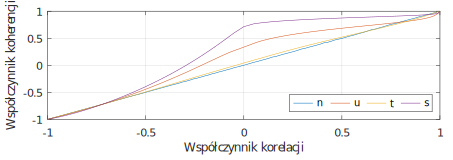
\includegraphics{obrazki/cohers}
\makecaption{fig:unc_cohers}{Zestawienie zależności wartości współczynników koherencji w funkcji współczynnika korelacji dla wybranych rodzajów rozkładu analizowanych sygnałów}
\end{center}
\end{figure}

Analizując przedstawione zależności zauważyć można, że sposób przedstawienia niedokładności wyniku pomiaru zależeć będzie w dużej mierze od potrzeb projektanta toru pomiarowego oraz od specyfiki zakłócających proces pomiaru błędów. Opis wykorzystujący wariancję błędów wydaje się bardziej przystępny, gdyż wariancja może być utożsamiana z mocą sygnału. Opis wykorzystujący niepewność rozszerzoną będzie jednak bardziej precyzyjny, natomiast wymaga większego zaangażowania w proces wyznaczania ostatecznej wartości tej niepewności. W odpowiednich okolicznościach, jeżeli spełnione są warunki związane z centralnym twierdzeniem granicznym, opis bazujący na wariancji błędu może być w łatwy sposób przeniesiony na opis związany z niepewnością rozszerzoną. Podczas wyznaczania wypadkowej wartości niepewności rozszerzonej stosować można metodę redukcyjnej arytmetyki interwałowej, opisaną szerzej w~\cite{jakubiec_reductive, jakubiec_arithmetic, jakubiec_redmono, batko_uncertainty}. Wyznaczone wartości niepewności rozszerzonej mogą w niewielkim stopniu odbiegać od wartości rzeczywistych, co opisano w~\cite{jakubiec_arithmetic, jakubiec_model}. Przyjmuje się jednak, że różnice nie przekraczające $5\%$ wartości prawdziwej są akceptowalne, przy czym bardziej korzystne są sytuacje gdzie błąd oszacowania cechuje się dodatnim znakiem -- tj. oszacowana wartość jest większa od rzeczywistej.

\section{Algorytm jako fragment toru pomiarowego}

Podczas opisu właściwości cyfrowej części toru pomiarowego przedstawiono przypadek, w którym analizowany obiekt przetwarzał kolejne próbki sygnału wejściowego na próbki sygnału wyjściowego zgodnie z odpowiadającą mu transmitancją i funkcją przetwarzania. Algorytmy stosowane w torach pomiarowych mogą generować wiele wielkości wyjściowych, pobierając przy tym w oknie pomiarowym określoną liczbę próbek wielkości wejściowych. W przypadku, gdy wyjście analizowanego obiektu stanowi $M$ próbek wielkości wyjściowych wyznaczanych na podstawie $N$ próbek wielkości wejściowych, a funkcja przetwarzania tego obiektu jest liniowa, działanie obiektu przedstawić można w ogólnej postaci jako~\cite{jakubiec_algorithms, jakubiec_single}:
\begin{equation}
\begin{bmatrix}
X \emb{0}   \\
X \emb{1}   \\
\vdots      \\
X \emb{M-1}
\end{bmatrix}
=
\begin{bmatrix}
a_{0, 0}   &   a_{0, 1} &   \cdots   &   a_{0, N-1}      \\
a_{1, 0}   &   \ddots   &            &   a_{1, N-1}      \\
\vdots     &            &   \ddots   &   \vdots          \\
a_{M-1, 0} &   \cdots   &   \cdots   &   a_{M-1, N-1}
\end{bmatrix}
\begin{bmatrix}
x \emb{0}   \\
x \emb{1}   \\
\vdots      \\
x \emb{N-1}
\end{bmatrix}
\label{eq:alg_out_mat},
\end{equation}
gdzie $a_{i,j}$ to kolejne współczynniki macierzy transformacji. Równanie~\eqref{eq:alg_out_mat} można przedstawić również w postaci iloczynu:
\begin{equation}
\mathbf{X} = \mathbf{A} \cdot \mathbf{x} \label{eq:alg_out_mul},
\end{equation}
gdzie $\mathbf{X}$ jest wektorem wielkości wyjściowych, $\mathbf{A}$ macierzą transformacji oraz $\mathbf{x}$ wektorem wielkości wejściowych~\cite{jakubiec_algorithms}. Wobec przedstawionych zależności, pojedynczą wielkość wyjściową algorytmu przedstawić można w postaci:
\begin{equation}
X \emb{i} = a_{i, 0} x \emb{0} + a_{i, 1} x \emb{1} + \hdots + a_{i, N-1} x \emb{N-1} \label{eq:alg_out_single}.
\end{equation}
Na podstawie przedstawionych zależności zauważyć można, że analizowany obiekt stanowi w zasadzie zbiór filtrów o skończonej odpowiedzi impulsowej \enquote{FIR}. Przedstawione metody analizy będą zatem przypominały metody analizy opisywanego typu filtru~\cite{mehrnia_fir}.

W praktyce wartości współczynników macierzy transformacji opisanej równaniem~\eqref{eq:alg_out_mat} mogą nie być znane przez projektanta toru pomiarowego. Ich znajomość jest jednak konieczna w celu przeprowadzenia analizy metrologicznej zastosowanego algorytmu. Najczęściej projektant toru pomiarowego stosuje gotowy algorytm, zaimplementowany np. w środowisku \enquote{GNU Octave} lub dostarczany mu jako zewnętrzną bibliotekę. W takim przypadku należy przeprowadzić proces identyfikacji wartości współczynników macierzy, który przedstawiony zostanie w dalszej części rozdziału. Innym przypadkiem jest sytuacja, w której z punktu widzenia analizy metrologicznej macierzowy opis algorytmu jest korzystny, a wartości współczynników mogą być wyznaczone za pomocą odpowiednich funkcjonałów. Ostatnim przypadkiem jest sytuacja, w której znana jest transmitancja $H(z)$ dla kolejnych wielkości wyjściowych. Wtedy wyznaczenie wartości współczynników macierzy transformacji odbywać się będzie poprzez przekształcenie tej transmitancji na postać zgodną z równaniem~\eqref{eq:alg_out_single}. Należy jednak zauważyć, że nie we wszystkich przypadkach przedstawione metody znajdują zastosowanie.

W przypadku, gdy dysponuje się gotową implementacją algorytmu, w celu identyfikacji współczynników macierzy transformacji należy podawać na wejście algorytmu wektor wielkości wejściowych, którego wszystkie elementy poza wybranym mają wartość zero. Wartość jednego elementu należy ustawić na jeden, a następnie za pomocą identyfikowanego algorytmu wyznaczyć należy wektor wielkości wyjściowych. Wyznaczony wektor stanowi kolumnę identyfikowanej macierzy transformacji, przy czym numer kolumny jest równy indeksowi elementu, który w wektorze wielkości wejściowych posiadał wartość jeden. W celu wyznaczenia wszystkich wartości macierzy transformacji należy powtórzyć powyższą czynność dla wektorów wartości wejściowych algorytmu zgodnie z zależnością~\cite{jakubiec_algorithms}:
\begin{equation}
x \emb{n} =
\begin{cases}
	1 & $gdy$~n = i \\
	0 & $gdy$~n \neq i
\end{cases}
\label{eq:wt_ident},
\end{equation}
dla $i$ w przedziale $<0;N-1>$, gdzie $i$ jest indeksem identyfikowanej kolumny macierzy transformacji. Niezależnie od struktury numerycznej analizowanego obiektu opisana metoda jest uniwersalna, przy czym wymaga ona, aby identyfikowany algorytm spełniał założenia przedstawione na początku podrozdziału.

Aby ustalić związek pomiędzy błędami wielkości wejściowych, a błędami wielkości wyjściowych analizowanego algorytmu należy przeanalizować proces wyznaczania wartości pojedynczej wielkości wyjściowej tego algorytmu. Wobec tego, jeżeli wielkości wejściowe algorytmu są obarczone błędami o charakterze addytywnym zgodnie z zależnością:
\begin{equation}
\tilde{x} \emb{i} = \dot{x} \emb{i} + e_{x,\Sigma} \emb{i} = \dot{x} \emb{i} + e_{x,s} \emb{i} + e_{x,d} \emb{i} + e_{x,r} \emb{i} \label{eq:alg_inputval},
\end{equation}
gdzie $e_{x,s}$ oznacza błąd statyczny, $e_{x,d}$ błąd dynamiczny oraz $e_{x,r}$ błąd losowy wielkości wejściowej, to istnieje możliwość osobnej analizy wyniku algorytmu dla idealnych wartości wielkości wejściowych oraz dla związanych z nimi błędów. Błąd wielkości wyjściowej przenoszony z wejścia na wyjście algorytmu można zatem opisać, zgodnie z równaniem~\eqref{eq:alg_out_single}, jako kombinację liniową współczynników transformacji algorytmu oraz błędów wielkości wejściowych:
\begin{equation}
e_{X,p} \emb{i} = a_{i, 0} e_{x,\Sigma} \emb{0} + a_{i, 1} e_{x,\Sigma} \emb{1} + \hdots + a_{i, N-1} e_{x,\Sigma} \emb{N-1} \label{eq:alg_outerr}.
\end{equation}

Dla błędów o charakterze statycznym, ze względu na fakt że realizacja tych błędów jest niezmienna w obrębie okna pomiarowego, równanie~\eqref{eq:alg_outerr} można uprościć i zapisać w postaci:
\begin{equation}
e_{X,s} \emb{i} = a_{i, 0} e_{x,s} + a_{i, 1} e_{x,s} + \hdots + a_{i, N-1} e_{x,s} = e_{x,s} \sum _{j = 0} ^{N-1} a_{i, j} \label{eq:alg_outerr_stat},
\end{equation}
gdzie $e_{x,s}$ jest błędem statycznym wielkości wejściowej, natomiast $e_{X,s}$ błędem statycznym wielkości wyjściowej algorytmu. Powtarzając pomiar wielokrotnie, dla różnych pozycji okna pomiarowego, realizacje błędu statycznego mogą przyjmować różne wartości. W takim przypadku wyjściowy błąd statyczny również można rozpatrywać w kategoriach probabilistycznych, a jego wariancję opisać można równaniem uwzględniającym wariancję wejściowego błędu statycznego:
\begin{equation}
\sigma_{X,s}^{2} \emb{i} = \sigma_{x,s}^{2} \left( a_{i, 0} + a_{i, 1} + \hdots + a_{i, N-1} \right)^{2} = \sigma_{x,s}^{2} \left( \sum _{j = 0} ^{N-1} a_{i, j} \right)^{2} \label{eq:alg_outvar_stat}.
\end{equation}
Należy zauważyć, że kształt rozkładu wyjściowego błędu statycznego będzie identyczny, jak kształt rozkładu statycznego błędu wejściowego.

Dla błędów o charakterze dynamicznym należy przeprowadzić analizę zgodnie z metodologią przedstawioną w poprzedniej części rozdziału, wykorzystując znajomość transmitancji $H(z)$ odpowiedniej dla analizowanej wielkości wyjściowej algorytmu. Identycznie, jak w przypadku równania~\eqref{eq:mid_disc_err_dyn_prop}, wyznaczyć należy wypadkowe amplitudy oraz przesunięcia w fazie kolejnych harmonicznych błędu dynamicznego, a następnie złożyć je zgodnie z zależnością~\eqref{eq:dyn_multi}. Transmitancja $H(z)$ dla $i$-tej wielkości wyjściowej może zostać wyznaczona na podstawie wartości współczynników $i$-tego wiersza macierzy transformacji algorytmu jako:
\begin{equation}
H_{i} \emb{z} = a_{i, 0} + a_{i, 1} z^{-1} + \hdots + a_{i, N-1} z^{-N+1} = \sum _{k = 0} ^{N-1} a_{i, k} z^{-k} \label{eq:alg_trans_single}.
\end{equation}
W omawianym przypadku przyjmuje się, że algorytm posiada idealną transmitancję, a ewentualne rozbieżności nie mają wpływu na widmo przenoszonego sygnału. Dodatkowe informacje związane z tym zagadnieniem zostaną przedstawione w dalszej części podrozdziału.

W przypadku błędów o charakterze losowym, wykonując algorytm wielokrotnie, uzyskać można zależność wiążącą wariancję błędu na wyjściu algorytmu z wariancją błędów wielkości wejściowych. Zakładając, że wszystkie wielkości wejściowe algorytmu pochodzą z tej samej cześć toru pomiarowego, a zatem ich parametry statystyczne są identyczne, oraz że kolejne błędy wielkości wejściowych nie są ze sobą skorelowane, zależność tą opisać można jako:
\begin{equation}
\sigma_{r}^{2} \emb{i} = a_{i, 0}^{2} \sigma_{x,r}^{2} + a_{i, 1}^{2} \sigma_{x,r}^{2} + \hdots + a_{i, N-1}^{2} \sigma_{x,r}^{2} = \sigma_{x,r}^{2} \sum _{j=0} ^{N-1} {a_{i, j}^{2}} \label{eq:alg_outvar_rand}.
\end{equation}

Poza przenoszeniem przez algorytm błędów zawartych w wielkościach wejściowych na jego wyjście, algorytm wprowadza do wielkości wyjściowych błędy własne. Błędy te wynikają niedokładności wyznaczenia współczynników algorytmu oraz z przeprowadzanych podczas obliczeń zaokrągleń. Ich wartości będą zatem uzależnione od wielu czynników, a ich analiza powinna odbywać się indywidualnie dla zaimplementowanego algorytmu. Zakładając, że wyznaczanie wartości $i$-tej wielkości wyjściowej algorytmu odbywać się będzie wielokrotnie, błędy własne opisywać można w kategorii probabilistycznej za pomocą związanej z nimi wariancji $\sigma_{X,z}^{2}(i)$. Ze względu na fakt, że liczba operacji mnożenia i dodawania, odpowiedzialnych za powstawanie omawianej grupy błędów będzie duża ($N$ mnożeń oraz $N$ dodawań) błąd ten będzie miał rozkład zbliżony do normalnego~\cite{jcgm_guide}. W przypadku, gdy na etapie identyfikacji wartości macierzy współczynników uzyskano wartości obarczone błędami, należy rozszerzyć analizę o przedstawienie konsekwencji tego zjawiska. W takim przypadku należy przeanalizować wprowadzany do wielkości wyjściowych statyczny błąd własny oraz wykonać analizę dla błędów własnych dynamicznych, analogicznie jak opisano równaniem~\eqref{eq:mid_disc_err_dyn_self}. Omawiany przypadek nie będzie rozpatrywany w pracy, ponieważ identyfikując wartości macierzy transformacji za pomocą przedstawionego algorytmu lub wyznaczając ich wartości przy użyciu odpowiednich funkcjonałów, wprowadzany błąd wynikać będzie głównie z zaokrągleń i będzie można analizować go równolegle z wprowadzanym losowym błędem $e_{X,z}$. Omawianą analizę przedstawia szczegółowo praca~\cite{jakubiec_system}.

Wobec powyższych założeń, w celu wyznaczenia wariancji $\sigma_{X,\Sigma}^{2}(i)$ wypadkowego błędu $e_{X,\Sigma}(i)$ dla $i$-tej wielkości wyjściowej analizowanego algorytmu należy wykorzystać zależność~\eqref{eq:var_matrix}, przy czym przyjmuje ona w tym przypadku postać:
\begin{equation}
\sigma_{X,\Sigma}^{2} \emb{i} =
\begin{bmatrix}
\sigma_{X,s} \emb{i} \\ \sigma_{X,d} \emb{i} \\ \sigma_{X,r} \emb{i} \\ \sigma_{X,z} \emb{i}
\end{bmatrix}^{T}
\begin{bmatrix}
1         & r_{d,s} & r_{r,s} & r_{z,s} \\
r_{s,d}   & 1       & r_{r,d} & r_{z,d} \\
r_{s,r}   & r_{d,r} & 1       & r_{z,r} \\
r_{s,z}   & r_{d,z} & r_{r,z} & 1
\end{bmatrix}
\begin{bmatrix}
\sigma_{X,s} \emb{i} \\ \sigma_{X,d} \emb{i} \\ \sigma_{X,r} \emb{i} \\ \sigma_{X,z} \emb{i}
\end{bmatrix}
\label{eq:alg_outvar_mat},
\end{equation}
gdzie $r_{i,j}$ stanowi współczynnik macierzy korelacji dla wybranych błędów cząstkowych analizowanego algorytmu. Wyznaczenie niepewności rozszerzonej może być przeprowadzone zgodnie z zależnością~\eqref{eq:unc_matrix}, przekształconą do postaci:
\begin{equation}
U_{X,\Sigma} \emb{i} = \sqrt{
\begin{bmatrix}
U_{X,s} \emb{i} \\ U_{X,d} \emb{i} \\ U_{X,r} \emb{i} \\ U_{X,z} \emb{i}
\end{bmatrix}^{T}
\begin{bmatrix}
1         & h_{d,s} & h_{r,s} & h_{z,s} \\
h_{s,d}   & 1       & h_{r,d} & h_{z,d} \\
h_{s,r}   & h_{d,r} & 1       & h_{z,r} \\
h_{s,z}   & h_{d,z} & h_{r,z} & 1
\end{bmatrix}
\begin{bmatrix}
U_{X,s} \emb{i} \\ U_{X,d} \emb{i} \\ U_{X,r} \emb{i} \\ U_{X,z} \emb{i}
\end{bmatrix}}
\label{eq:alg_outunc_mat},
\end{equation}
przy czym $h_{i,j}$ oznacza współczynnik koherencji wyznaczany zgodnie z zależnością~\eqref{eq:unc_coher}. Należy zauważyć, że równania~\eqref{eq:alg_outvar_mat} oraz~\eqref{eq:alg_outunc_mat} mogą zawierać więcej elementów składowych, niż wskazano. Dokładna postać przedstawionych równań zależeć będzie od budżetu niepewności wielkości wejściowych analizowanego algorytmu.

Na podstawie równań~\eqref{eq:alg_outvar_stat} oraz~\eqref{eq:alg_outvar_rand} wprowadzić można dodatkowe wielkości przedstawione następującymi zależnościami:
\begin{gather}
A_{i,s} = \sum _{j = 0} ^{N-1} a_{i, j} \label{eq:alg_trans_stat}, \\
A_{i,r} = \sqrt{\sum _{j = 0} ^{N-1} a_{i, j}^{2}} \label{eq:alg_trans_rand},
\end{gather}
gdzie $A_{i,s}$ jest współczynnikiem przenoszenia dla błędów statycznych, natomiast jest $A_{i,r}$ współczynnikiem przenoszenia dla błędów losowych $i$-tej wielkości wyjściowej analizowanego algorytmu. Wyznaczenie wartości opisanych współczynników umożliwi wyznaczenie wariancji kolejnych błędów losowych oraz statycznych, a dodatkowo będzie stanowiło informacje, w jaki sposób analizowany algorytm przenosi z wejścia na wyjście określony rodzaj błędu. Można zauważyć, że dla niskich wartości współczynnika przenoszenia (tj. $A_{i} < 1$) kolejne błędy wielkości wejściowych będą tłumione (wariancja błędu wielkości wyjściowej będzie mniejsza, niż wariancja błędów wielkości wejściowych). Odwrotna sytuacja będzie miała miejsce w przypadku dużych wartości współczynnika (tj. $A_{i} > 1$).

W przypadku analizy błędów dynamicznych, na podstawie równania~\eqref{eq:alg_trans_single} po podstawieniu $z = e^{j\omega}$, wyznaczyć można adekwatne dla równań~\eqref{eq:mid_disc_amp} oraz~\eqref{eq:mid_disc_phi} zależności opisujące wzmocnienie $K_{X,i}(\omega_{n})$ oraz przesunięcie w fazie $\varphi_{X,i}(\omega_{n})$ przetwarzanych harmonicznych sygnału w funkcji pulsacji znormalizowanej $\omega_{n}$ dla $i$-tej wielkości wyjściowej algorytmu w postaci:
\begin{gather}
G_{X,i} \emb{\omega_{n}} = \sum _{k = 0} ^{N-1} a_{i,k} e^{-j k \omega_{n}} \label{eq:alg_trans_norm}, \\
K_{X,i} \emb{\omega_{n}} = \left| G_{X,i} \emb{\omega_{n}} \right| = \sqrt{\left( \Re \left( G_{X,i} \emb{\omega_{n}} \right) \right)^{2} + \left( \Im \left( G_{X,i} \emb{\omega_{n}} \right) \right)^{2}} \label{eq:alg_trans_amp}, \\
\varphi_{X,i} \emb{\omega_{n}} = \arctan \left( \frac{\Im \left( G_{X,i} \emb{\omega_{n}} \right)}{\Re \left( G_{X,i} \emb{\omega_{n}} \right)} \right) \label{eq:alg_trans_phi},
\end{gather}
przy czym pulsacja znormalizowana, oznaczona symbolem $\omega_{n}$, odnosi się do pulsacji próbkowania i jest określona przez następującą zależność:
\begin{equation}
\omega_{n} = 2\pi \frac{\omega}{\omega_{s}} \label{eq:puls_norm},
\end{equation}
gdzie $\omega$ jest analizowaną pulsacją, natomiast $\omega_{s}$ pulsacją próbkowania równą $\frac{2 \pi}{T_{p}}$ dla okresu próbkowania $T_{p}$. Prawidłowa wartość pulsacji znormalizowanej mieści się zatem w zakresie $<0;\pi>$, co odpowiada zakresowi od zera do pulsacji Nyquista dla przyjętego okresu próbkowania.

\section{Podsumowanie przedstawionych zależności}

W poprzednich częściach rozdziału przedstawiono modele kolejnych fragmentów toru pomiarowego, które opisywały związki pomiędzy błędami na wejściu i wyjściu analizowanego obiektu, a także wskazywały rolę tego obiektu we wprowadzaniu do sygnału wyjściowego błędów własnych. Zaproponowany model wprowadzał podział na statyczne i dynamiczne właściwości obiektu, które opisywane były transmitancją i funkcją przetwarzania obiektu. Opisane zaproponowanym modelem fragmenty toru pomiarowego, które zostały ze sobą połączone kaskadowo oraz cechują się addytywną funkcją przetwarzania, opisać można modelem wypadkowym oraz z osobna analizować zawarte w nim błędy cząstkowe. Zaproponowana metoda wyznaczania niepewności wypadkowej bazuje na określeniu związków pomiędzy kolejnymi niepewnościami składowymi, a następnie wykorzystuje redukcyjną arytmetykę interwałową do wyznaczenia niepewności wypadkowej. Zaproponowany opis uwzględnia ewentualne korelacje pomiędzy kolejnymi grupami błędów, a w przypadku braku tych korelacji wymaga jedynie określenia związków pomiędzy kształtem rozkładu kolejnych składanych błędów~\cite{jakubiec_reductive, batko_uncertainty}.

Przedstawiony model oceny dokładności wyniku pomiaru zakłada, że obecne w sygnale pomiarowym błędy cechują się symetrycznymi rozkładami o zerowej wartości oczekiwanej. W przypadku, gdy wartość oczekiwana realizacji błędu jest niezerowa, błąd ten posiada składową systematyczną, którą należy skorygować w ostatecznym wyniku pomiaru. Jeżeli nie jest spełnione założenie odnośnie symetrii rozkładów składanych błędów, to do określenia rozkładu błędu wynikowego należy stosować metodę analityczną bazującą na wyznaczeniu splotu składanych funkcji gęstości prawdopodobieństwa lub wykorzystać metodę Monte-Carlo, która jest zwykle bardziej przystępna i optymalna ze względu na mniejszy stopień skomplikowania~\cite{janssen_montecarlo, roj_annuncertainty}.

Przeprowadzone rozważania nie poruszały problemu opóźnień w systemach pomiarowo-sterujących, a zatem nie brano w nich pod uwagę błędów związanych z opóźnieniami. Tematyka ta nie będzie poruszana w dalszych częściach pracy. Warto jednak zauważyć, że zaproponowany model błędu może być z łatwością dopasowany do możliwości analizy właściwości i wpływu tych błędów na niedokładność wielkości wyjściowych. Należy wtedy uwzględnić w modelu dodatkowy składnik błędu, który definiować można zgodnie z metodą zaproponowaną w~\cite{wymyslo_delay, jakubiec_system}. Z punktu widzenia zaproponowanego modelu, zjawisko to opisać można jako dodatkowe przesunięcie w fazie składowych przetwarzanego sygnału, będące iloczynem pulsacji analizowanej harmonicznej i wartości realizacji błędu opóźnienia.
